%%%%%%%% ICML 2026 EXAMPLE LATEX SUBMISSION FILE %%%%%%%%%%%%%%%%%

\documentclass{article}

% Recommended, but optional, packages for figures and better typesetting:
\usepackage{microtype}
\usepackage{graphicx}
\usepackage{subcaption}
\usepackage{booktabs} % for professional tables

% hyperref makes hyperlinks in the resulting PDF.
% If your build breaks (sometimes temporarily if a hyperlink spans a page)
% please comment out the following usepackage line and replace
% \usepackage{icml2026} with \usepackage[nohyperref]{icml2026} above.
\usepackage{hyperref}


% Attempt to make hyperref and algorithmic work together better:
\newcommand{\theHalgorithm}{\arabic{algorithm}}

% Use the following line for the initial blind version submitted for review:
% \usepackage{icml2026}

% For preprint, use
\usepackage{icml2026}

% If accepted, instead use the following line for the camera-ready submission:
% \usepackage{icml2026}

\usepackage{amsmath}
\usepackage{amssymb}
\usepackage{mathtools}
\usepackage{amsthm}


% if you use cleveref..
\usepackage[capitalize,noabbrev]{cleveref}








\usepackage{float}
\usepackage{placeins}

\usepackage{pifont}
\usepackage{amssymb}

\usepackage{booktabs}						% professional-quality tables
\usepackage{multirow}						% tabular cells spanning multiple rows
\usepackage{amsfonts}						% blackboard math symbols
\usepackage{graphicx}						% figures
\usepackage{duckuments}						% sample images
\usepackage{wrapfig}
\usepackage{amssymb}


\usepackage{listings}
\usepackage{xcolor}
\usepackage[most]{tcolorbox}
\usepackage{courier} % 可选：代码字体更像等宽
\usepackage{lipsum}
\usepackage{siunitx}

\usepackage{caption}
\usepackage{multirow}
\usepackage{bm}
\usepackage{amsmath}
\usepackage{amsfonts}
% \usepackage{amssymb}

\usepackage{marginnote}









%%%%%%%%%%%%%%%%%%%%%%%%%%%%%%%%
% THEOREMS
%%%%%%%%%%%%%%%%%%%%%%%%%%%%%%%%
\theoremstyle{plain}
\newtheorem{theorem}{Theorem}[section]
\newtheorem{proposition}[theorem]{Proposition}
\newtheorem{lemma}[theorem]{Lemma}
\newtheorem{corollary}[theorem]{Corollary}
\theoremstyle{definition}
\newtheorem{definition}[theorem]{Definition}
\newtheorem{assumption}[theorem]{Assumption}
\theoremstyle{remark}
\newtheorem{remark}[theorem]{Remark}

% Todonotes is useful during development; simply uncomment the next line
%    and comment out the line below the next line to turn off comments
%\usepackage[disable,textsize=tiny]{todonotes}
\usepackage[textsize=tiny]{todonotes}










\DeclareMathOperator*{\argmax}{arg\max}



\usepackage{times}
\usepackage{latexsym}

% For proper rendering and hyphenation of words containing Latin characters (including in bib files)
\usepackage[T1]{fontenc}
% For Vietnamese characters
% \usepackage[T5]{fontenc}
% See https://www.latex-project.org/help/documentation/encguide.pdf for other character sets

% This assumes your files are encoded as UTF8
\usepackage[utf8]{inputenc}

% This is not strictly necessary, and may be commented out,
% but it will improve the layout of the manuscript,
% and will typically save some space.
\usepackage{microtype}

% This is also not strictly necessary, and may be commented out.
% However, it will improve the aesthetics of text in
% the typewriter font.
\usepackage{inconsolata}

%Including images in your LaTeX document requires adding
%additional package(s)
\usepackage{graphicx}



















% The \icmltitle you define below is probably too long as a header.
% Therefore, a short form for the running title is supplied here:
\icmltitlerunning{Revisiting RAG Retrievers: An Information Theoretic Benchmark}

\begin{document}

\twocolumn[
  \icmltitle{Revisiting RAG Retrievers: An Information Theoretic Benchmark}

  % It is OKAY to include author information, even for blind submissions: the
  % style file will automatically remove it for you unless you've provided
  % the [accepted] option to the icml2026 package.

  % List of affiliations: The first argument should be a (short) identifier you
  % will use later to specify author affiliations Academic affiliations
  % should list Department, University, City, Region, Country Industry
  % affiliations should list Company, City, Region, Country

  % You can specify symbols, otherwise they are numbered in order. Ideally, you
  % should not use this facility. Affiliations will be numbered in order of
  % appearance and this is the preferred way.
  \icmlsetsymbol{equal}{*}

  \begin{icmlauthorlist}\icmlauthor{Anonymous}{anon}\end{icmlauthorlist}
  % \icmlaffiliation{anon}{Anonymous Institution}
  
  % 

  \icmlcorrespondingauthor{Anonymous}{anonymous@anonymous.invalid}
  % 


  % You may provide any keywords that you find helpful for describing your
  % paper; these are used to populate the "keywords" metadata in the PDF but
  % will not be shown in the document
  \icmlkeywords{Machine Learning, ICML}

  \vskip 0.3in
]

% this must go after the closing bracket ] following \twocolumn[ ...

% This command actually creates the footnote in the first column listing the
% affiliations and the copyright notice. The command takes one argument, which
% is text to display at the start of the footnote. The \icmlEqualContribution
% command is standard text for equal contribution. Remove it (just {}) if you
% do not need this facility.

% Use ONE of the following lines. DO NOT remove the command.
% If you have no special notice, KEEP empty braces:
\printAffiliationsAndNotice{}  % no special notice (required even if empty)
% Or, if applicable, use the standard equal contribution text:
% \printAffiliationsAndNotice{\icmlEqualContribution}

\begin{abstract}
Retrieval-Augmented Generation (RAG) systems rely critically on the retriever module to surface relevant context for large language models. Although numerous retrievers have recently been proposed, each built on different ranking principles such as lexical matching, dense embeddings, or graph citations, there remains a lack of systematic understanding of how these mechanisms differ and overlap. Existing benchmarks primarily compare entire RAG pipelines or introduce new datasets, providing little guidance on selecting or combining retrievers themselves. Those that do compare retrievers directly use a limited set of evaluation tools which fail to capture complementary and overlapping strengths. This work presents MIGRASCOPE, a Mutual Information based RAG Retriever Analysis Scope. We revisit state-of-the-art retrievers and introduce principled metrics grounded in information and statistical estimation theory to quantify retrieval quality, redundancy, synergy, and marginal contribution. We further show that if chosen carefully, an ensemble of retrievers outperforms any single retriever. We leverage the developed tools over major RAG corpora to provide unique insights on contribution levels of the state-of-the-art retrievers. Our findings provide a fresh perspective on the structure of modern retrieval techniques and actionable guidance for designing robust and efficient RAG systems.

\end{abstract}




\section{Introduction}


Retrieval-Augmented Generation (RAG) has emerged as a dominant paradigm for knowledge-intensive NLP tasks \cite{lewis2020retrieval}. By retrieving relevant external context to inform large language models (LLMs), RAG systems dramatically improve factual accuracy and reduce hallucination \cite{shuster2021retrieval}. The retriever module is the core component responsible for selecting which evidence is passed to the generator, and its effectiveness directly limits downstream performance. A rich ecosystem of retrievers has flourished, including lexical-based methods such as BM25 \cite{robertson2009probabilistic}, dense embedding models trained for semantic similarity \citep{karpukhin2020dense}, graph-based retrievers designed for multi-hop and global reasoning \citep{edge2024local}, and increasingly hybrid retrieval systems \cite{sarmah2024hybridrag} . Each introduces distinct assumptions and ranking mechanisms, yet the field lacks a unified framework to compare them rigorously. % Beyond standard ranking metrics such as recall, precision, and ndcg that rely on binary ...
Many existing benchmarks focus on new datasets or evaluation metrics applied to full RAG pipelines. While these studies provide valuable insights into overall system quality, they rarely isolate retrieval performance. 
Some retriever-specific evaluation work has been done, covering heterogeneous domain generalization \cite{thakur2021beir}, massive embedding leaderboards \cite{muennighoff2023mteb}, and complex-objective tasks \cite{wang2024birco}. However these frameworks focus on aggregate ranking-based metrics such as recall, MRR, and nDCG which assume independence between retrieved items and thus  fail to explain how different retrievers complement or supersede each other. 
Recent ensemble-RAG efforts mostly concentrate on hierarchical integration of the full pipeline without disentangling the unique contributions of the retriever itself. As a result, practitioners face uncertainty when selecting the best retriever for a given application or dataset, and new retrievers are introduced without clarity about the retrieval behaviors they replace or replicate. We argue that revisiting the retriever module with dedicated evaluation tools is essential to unlocking the next phase of RAG progress.

% While ranking metrics like nDCG reward the correct ordering of documents, they are invariant to the probability mass assigned to them. Our divergence-based metric penalizes retrievers that are correctly ranked but semantically miscalibrated—such as those that over-represent a single facet of an answer while marginalizing equally important complementary evidence.

% \subsection{Illustrative Example: Rank-order vs. Distributional Alignment  }
% To understand why a divergence-based metric is necessary alongside standard ranking metrics, consider a query $q$ that requires a multifaceted answer. For example, "What are the pros and cons of product X?" Let the pseudo-ground-truth distribution $CP^*$ derived from the answer assign equal importance to two distinct chunks: a "Pro" chunk ($c_1$) and a "Con" chunk ($c_2$).$$CP^*(c | q, a) \approx \{c_1: 0.5, c_2: 0.5\}$$Now consider two hypothetical retrievers that both successfully identify these chunks as the top two results, but with different predicted confidence scores $p_A$ and $p_B$:  
% \begin{itemize}
%     \item Retriever A (Balanced): Assigns equal scores to both chunks.
%     \begin{itemize}
%         \item $p_A$: $\{c_1: 0.5, c_2: 0.5\}$.
%         \item Ranking: 1. $c_1$, 2. $c_2$.
%     \end{itemize}
%     \item Retriever B (Skewed): Assigns a high score to the "Pro" and a barely non-zero score to the "Con."
%     \begin{itemize}
%         \item $p_B$: $\{c_1: 0.99, c_2: 0.01\}$.
%         \item Ranking: 1. $c_1$, 2. $c_2$.
%     \end{itemize}
% \end{itemize}
% \textbf{Under nDCG}: Both retrievers receive the exact same score. It treats the negligible probability assigned to $c_2$ by Retriever B as irrelevant, provided $c_2$ is still ranked second.   

% \noindent \textbf{Under JSD (Our Metric)}: The two retrievers receive drastically different scores.  
% \begin{itemize}
%     \item Retriever A achieves $JSD(p_A || CP^*) \approx 0$ (High Quality). 
%     \item Retriever B achieves a high divergence score (Low Quality) because its probability mass fails to reflect the balanced nature of the required information.  
% \end{itemize}
% Traditional metrics like nDCG assume a human user browsing a list linearly; as long as the relevant document is "visible" (i.e. ranked high), the absolute score is irrelevant. In contrast, RAG systems ingest the retrieved context entirely. A retriever that is "technically correct" in ranking but highly skewed in probability distribution (like Retriever B) signals a false certainty. In practice, such skew often manifests as the retriever filling the top-$k$ slots with redundant variations of $c_1$ while pushing $c_2$ out of the context window entirely. 

% A divergence-based metric enforces distributional alignment, ensuring that the retrieved context mirrors the informational spread of the ground truth. By penalizing mis-calibration, our framework favors retrievers that not only find the right answers but represent them with the correct semantic proportions, reducing the likelihood of generator hallucination or bias.

To address these gaps, we introduce MIGRASCOPE, an information-theoretic framework for analyzing and benchmarking retrievers in RAG. We model each retriever’s ranking signal as a noisy view of an underlying chunk probability distribution conditioned on ground-truth answers. Building on Mutual Information (MI), we define a retriever quality score that computes the diverging level from the presumed ideal chunk distribution. This score generalizes across lexical, dense, and graph-based retrieval mechanisms, enabling principled comparison and calibration.

We further develop MI-grounded synergy and redundancy metrics to quantify how multiple retrievers interact—whether they contribute complementary evidence or duplicate signals—and provide visual diagnostics to reveal overlap structure. These tools support marginal contribution estimation and guide retriever selection and combination.

Finally, we translate these analyses into practice with a lightweight ensemble that uses MI-based attribution to select and weight retrievers with minimal supervision. Applied across major RAG corpora and a broad suite of state-of-the-art (SOTA) retrievers, the framework yields new insights into contribution patterns, redundancy, and robustness, and the ensemble consistently outperforms strong single retrievers. This paper makes the following contributions:

\begin{itemize}
% \vspace{-0.5em}
\item Introduce MIGRASCOPE, a mutual-information–based retriever quality score that normalizes across ranking paradigms (lexical, dense, graph) to quantify retrieval relevance and utility.
% \vspace{-0.5em}
\item Define and visualize MI-grounded synergy and redundancy metrics for multiple retrievers, revealing complementary and overlapping signal structure within ensembles.
% \vspace{-0.5em}
\item Develop a retriever ensemble framework with MI-based attribution to estimate each retriever’s marginal contribution to overall retrieval performance.
% \vspace{-0.5em}
\item Benchmark a broad set of graph-RAG and standard RAG retrievers using the proposed methodology, yielding new insights on contribution patterns, robustness, and design guidance for RAG systems.
\end{itemize}
% \vspace{-0.5em}

Our results suggest a need to shift community focus from endlessly inventing new retrievers toward understanding how existing ones differ, overlap, and cooperate. Through an information-theoretic lens, we uncover structure and simplicity hidden beneath the diversity of modern retrieval methods, paving the way for more reliable and interpretable RAG systems.






\begin{figure*}[h]
    \centering
    \renewcommand{\thefigure}{A}
    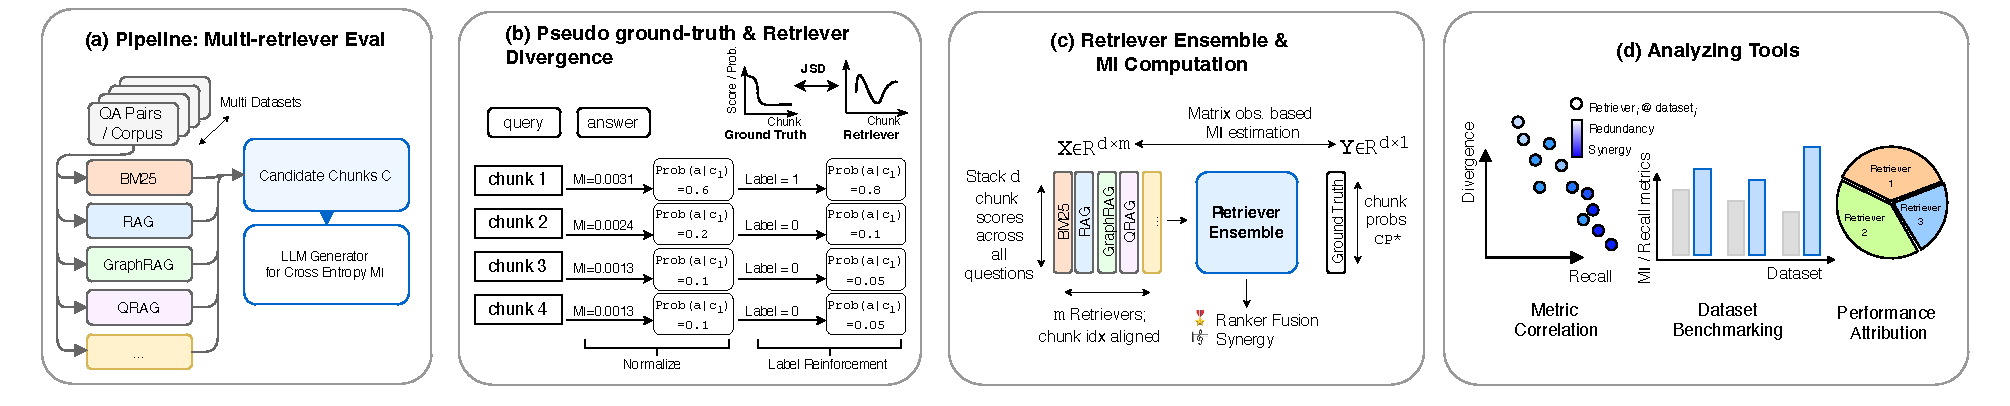
\includegraphics[trim=1.5em 0.8em 1.7em 0.2em, clip,width=0.97\linewidth]{figs/qrag.pdf}
    \caption{The proposed MIGRASCOPE analyzing framework}
    % (This figure is to be re-worked: \url{https://drive.google.com/file/d/1Runx3SIDHHCxbxAUpPA7X3hv4zpKmIz7/view?usp=sharing} -- WZ).}
    \label{fig:arch}
    % \vspace{-1em}
\end{figure*}





\section{Related Work}
\label{sec:related_work}

Our work is positioned at the intersection of three active research areas: RAG benchmarking, RAG ensemble methods, and the application of information-theoretic principles to large language models.

\subsection{RAG Benchmarking}
Recent work on RAG evaluation has primarily focused on establishing new datasets, defining system-level metrics, or analyzing operational costs, rather than systematically comparing the retrievers themselves. Several benchmarks have been introduced to test RAG systems on complex tasks, such as multi-hop reasoning over structured documents \citep{khang2025crest} or domain-specific GraphRAG applications \citep{xiao2025graphrag}. Others have focused on creating datasets for specific industrial domains, such as finance \citep{wang2024omnieval}, or on proposing new evaluation methodologies, like assessing LLM robustness and information integration \citep{chen2024benchmarking} or developing explainable metrics for industrial settings \citep{friel2024ragbench}.

To evaluate retrievers in isolation, the Information Retrieval community has developed rigorous benchmarks covering heterogeneous domain generalization \citep{thakur2021beir}, massive embedding leaderboards \citep{muennighoff2023mteb}, and complex user objectives \citep{wang2024birco}. However, these frameworks typically rely on aggregate ranking metrics such as nDCG and Recall. While effective for static leaderboards, these metrics treat document utility as additive, implicitly assuming independence between retrieved items. Consequently, they fail to quantify redundancy or measure the conditional information gain required to understand how distinct retrievers complement or supersede one another in an ensemble.

While valuable, these contributions often treat the retriever as a component within a larger pipeline. The focus remains on dataset design or system-level assessment. Other studies analyze important, but orthogonal, aspects. For instance, \citet{lin2024operational} provide practical guidance on the operational trade-offs of different retrieval infrastructures (e.g., HNSW vs. inverted indexing) but do not offer prescriptive insights on retriever algorithm selection. Similarly, \citet{zhang2025comparative} compare different LLMs as dense retrievers, but limit their analysis to this single family. 

Across these studies, there remains a significant gap in understanding the fundamental differences, redundancies, and complementary strengths of the various retriever families (e.g., dense, sparse, hybrid, and graph-based). Our work directly addresses this gap by proposing a framework to benchmark the retrievers themselves.

% \vspace{-1em}
\subsection{RAG Ensemble Methods}
% \vspace{-0.5em}
As RAG systems have matured, ensemble and multi-retriever architectures have become increasingly common. Many of these efforts focus on sophisticated pipeline orchestration. For example, \citet{zhang2025levelrag} propose a hierarchical system with a planner that orchestrates multiple low-level searchers, while \citet{wu2025composerag} introduce a modular framework that composes distinct steps like question decomposition and retrieval. Other approaches integrate heterogeneous data sources, such as combining web search with knowledge graphs \citep{xie2024weknow} or creating adaptive hybrid systems for specific domains like law \citep{kalra2024hypa}.

A separate line of work seeks to optimize the information passed to the generator. This includes methods for decoupling retrieval and generation representations \citep{yang2025heterag} or explicitly balancing relevance and semantic diversity in the retrieved document set \citep{rezaei2025vendi}. \citet{chen2025revisiting} explicitly analyze ensembles through an information-theoretic lens, arguing that they increase the total useful information. However, their work stops short of providing an operational recipe for selecting or weighting retrievers. These studies primarily offer architectural solutions or in-domain systems, but do not provide a principled, data-driven method for understanding \emph{which} retrievers to ensemble or \emph{how} to combine them based on their quantified marginal contribution.

% \vspace{-1em}
\subsection{Information-Theoretic Analysis in RAG}
% \vspace{-0.5em}
Information theory provides a powerful, formal toolkit for quantifying concepts like uncertainty, relevance, and redundancy, which are central to RAG. Recently, these tools have been applied to various parts of the RAG pipeline. For instance, \citet{zhu2024information} use an information bottleneck formulation to filter noise from retrieved contexts. \citet{liu2024pointwise} propose using Pointwise Mutual Information (PMI) as a probabilistic gauge for RAG performance, while others have used divergence metrics to measure attribution \citep{li2025attributing} or detect hallucinations \citep{halperin2025prompt}. These methods successfully apply information-theoretic concepts to \emph{diagnose} or \emph{optimize} a specific RAG component, such as context pruning \citep{deng2025influence} or detecting data memorization \citep{anh2025repcs}.

However, this body of work has not yet been directed at the problem of \emph{retriever evaluation}. While \citet{yumucsak2025information} outline a theoretical framework for RAG information flow, it lacks the empirical benchmarking to reveal how different SOTA retrievers actually perform under these metrics. To our knowledge, no existing work uses mutual information and information divergence to create a comparative framework that quantifies the quality, redundancy, and marginal contribution of distinct retriever families.

In summary, the field currently lacks a unified framework for comparing retriever modules directly, a principled method for designing retriever ensembles based on redundancy, and an empirical application of information theory to benchmark retriever contributions. Our work, MIGRASCOPE, is designed to fill these precise gaps.




% \section{Literature Review (WIP...)}

% \subsection{RAG Benchmark Related Papers}

% \cite{lin2024operational} studies the operational trade-offs between dense and sparse retrieval infrastructures, including HNSW, flat, and inverted indexing, providing practical deployment guidance under different corpus scales. However, its analysis centers on indexing cost and retrieval latency rather than offering prescriptive insights about which retriever architecture is optimal for a new RAG scenario. The work does not include end-to-end RAG performance nor modern GraphRAG methods, leaving the question of retriever selection for novel tasks largely unanswered.

% \cite{zhang2025comparative} compares multiple specialized LLM variants as dense retrievers and reveals that domain specialization can lead to substantial retrieval performance variance. Although this work brings direct comparison of retriever options, it evaluates only dense retrievers and does not involve full RAG pipelines or hybrid/graph retrieval methods. The absence of latest RAG or GraphRAG numerical comparisons limits its practical value in guiding retriever choice for real-world applications.

% \cite{chen2024benchmarking} introduces a systematic RAG evaluation framework focusing on LLM robustness, information integration, negative filtering, and counterfactual grounding. The benchmark contributes structured evaluation methodology, yet it largely abstracts away the retriever design space. Different retrieval approaches are not compared in depth, and no actionable recommendation is provided regarding which retriever performs best in unseen tasks or domains.

% \cite{friel2024ragbench} proposes explainable RAG evaluation metrics across industrial settings and multiple domains, emphasizing diagnostic interpretability. Despite its strong evaluation contributions, the benchmark does not thoroughly analyze dense, sparse, or graph retrieval mechanisms. It thus cannot inform practitioners on retriever selection strategies beyond generic performance reporting.

% \cite{khang2025crest} targets complex reasoning over structured documents in RAG, advancing evaluation difficulty and multilingual applicability. The focus remains on dataset design and system-level assessment instead of retriever technology. Consequently, sparse, dense, and GraphRAG retrievers are not systematically compared, leading to limited ability to recommend retrieval approaches for these complex reasoning tasks.

% \cite{xiao2025graphrag} establishes a benchmark for domain-specific GraphRAG evaluation across multiple reasoning types and knowledge graph structures. Although it is closest to connecting retriever designs with downstream reasoning, the work still frames itself primarily as a benchmark rather than comprehensive retriever comparison research. It does not yield generalized principles for choosing between graph retrieval and alternative retrievers when facing a novel task.

% \cite{wang2024omnieval} develops a financial-domain RAG benchmark with automatic data generation and granular scenario classification. While valuable for vertical domain evaluation, it does not contribute extensive retriever comparisons nor prescribe optimal retriever configurations. As with other benchmarks, RAG performance is reported without systematic retrieval-level insights.

% \noindent\textbf{Summary:} Across all these studies, the primary contributions are benchmarks, datasets, or evaluation methodologies rather than systematic guidance for retriever selection. There remains a clear and significant gap in empirical understanding of how different retriever families (dense, sparse, hybrid, and graph-based) should be chosen or combined for new RAG/GraphRAG tasks with varying domains, corpus structures, and reasoning demands.




% \subsection{RAG Ensemble papers}

% \noindent \cite{rezaei2025vendi} proposes an iterative RAG pipeline that explicitly balances semantic diversity and answer quality: it measures inter-document diversity with the Vendi Score and couples retrieval with an LLM judge to up-weight document sets that jointly improve multi-hop reasoning accuracy across HotpotQA, 2WikiMultiHopQA, and MuSiQue; although this yields notable end-to-end gains, the method treats the retriever largely as a controllable diversity/relevance knob and does not offer a head-to-head analysis of alternative retriever families or guidance on which retrievers are superior under different tasks or corpora.

% \noindent \cite{zhang2025levelrag} decomposes complex queries via a high-level searcher and orchestrates multiple low-level searchers (sparse, dense, and web) through rewriting-based multi-hop planning, reducing tight coupling between query rewriting and a single dense retriever; despite demonstrating stronger corpus coverage and reasoning breadth, the work centers on planner–searcher integration and does not systematically compare retriever algorithms or yield practical prescriptions for choosing among dense, sparse, or hybrid retrievers beyond the proposed planner.

% \noindent \cite{yang2025heterag} introduces a heterogeneous RAG framework that decouples chunk representations between retrieval and generation—using context-enriched, multi-granular views for retrieval while keeping generation-oriented short chunks, plus adaptive prompt tuning for the retriever—improving both efficiency and grounding; yet the contribution primarily optimizes representational interfaces around a chosen retriever, without a comparative evaluation that would indicate when particular retriever models (dense vs. sparse vs. hybrid) are preferable.

% \noindent \cite{wu2025composerag} proposes a modular, composable multi-hop RAG that isolates question decomposition, rewriting, retrieval decision, reranking, and verification with prompt-mediated interfaces and self-reflection; while this architecture improves interpretability and grounding under identical retrieval conditions, the study largely fixes retrieval choices during experiments and does not use the modularity to derive actionable conclusions about which retriever types or configurations are most effective across datasets.

% \noindent \cite{chen2025revisiting} analyzes multi-RAG ensembles through information-theoretic and mechanistic lenses across pipeline and module levels, arguing that ensembles can increase useful information relative to single systems and exploring several collaboration patterns; however, aside from an entropy-based justification that ensemble knowledge can be more informative, there is no operational recipe for selecting the right subset of chunks from pooled retrievals nor a comparative study that identifies which retriever families should be included or excluded in practice.

% \noindent \cite{kalra2024hypa} targets legal/policy QA with a hybrid parameter-adaptive system that classifies query complexity to tune RAG parameters on the fly and integrates dense, sparse, and knowledge-graph retrieval under a tailored evaluation for NYC LL144; even though this domain system improves fidelity via adaptive control and heterogeneous sources, it emphasizes in-domain orchestration rather than a principled comparison of retriever models or recommendations about when each retriever is optimal.

% \noindent \cite{xie2024weknow} fuses live web search with knowledge-graph grounding inside a single RAG pipeline to curb hallucinations and improve factuality by combining structured KG signals with dense retrieval; while effective as a system-level integrator, it does not disentangle the contribution or relative merits of alternative retrievers, leaving open the question of which retriever architectures should be preferred or combined for new domains.



% \subsection{Information Entropy Related Papers}

% \cite{zhu2024information} introduces an information bottleneck (IB) formulation for RAG noise filtering by optimizing a query-conditioned chain that compresses retrieved chunks while preserving information relevant to the final answer. This work demonstrates improvements through context compression, yet it remains focused on filtering instead of benchmarking modern retrievers under IB metrics. Without systematic comparison across retriever families, the framework stops short of revealing which retrieval mechanism best preserves task-relevant mutual information on real datasets.

% \cite{liu2024pointwise} proposes pointwise mutual information between query and context as a probabilistic gauge for RAG performance, and further shows that PMI can be approximated using LLM perplexity-based likelihoods. Although this establishes a practical signal for context utility, the method is validated at the level of prompt reconstruction rather than comparative assessment among dense, sparse, hybrid, or graph-based retrievers. Therefore, PMI remains an indicator without accompanying evidence about which retriever maximizes it reliably.

% \cite{deng2025influence} defines a per-chunk Contextual Influence (CI) score to quantify the impact of removing individual evidence pieces, and distills this signal into a lightweight selector to prune irrelevant chunks. This aligns with the general idea of chunk-level contribution grounded in likelihood shifts, but attribution is localized and does not extend to identifying the superior retrieval approach across tasks or domains.

% \cite{li2025attributing} studies mechanistic context attribution using Jensen-Shannon divergence to capture distributional shifts in generation when specific sentences are masked. While offering a principled divergence-based measurement for evidence contribution, the work focuses on internal attribution rather than inter-retriever performance differences, leaving open the question of which retrieval strategy yields the most influential context in the first place.

% \cite{anh2025repcs} develops RePCS to diagnose data memorization in RAG via divergence comparisons of model behaviors with and without retrieval, providing safety auditing capabilities. Its relevance to retriever evaluation is indirect because it does not differentiate retrievers on information-retention or utility grounds.

% \cite{ren2025effective} introduces an RL-based transparent and robust RAG training paradigm featuring adaptive rewards and decision traceability. The contribution aims at generation-level robustness rather than information-theoretic analysis of retriever effectiveness.

% \cite{yumucsak2025information} outlines a theoretical information-theoretic framework for RAG pipelines, elucidating how information flows through retrieval and generation modules. The work is largely conceptual and lacks empirical benchmarking that would reveal how theoretical quantities vary across advanced retrievers.

% \cite{halperin2025prompt} proposes prompt–response semantic divergence metrics for hallucination and misalignment detection, capturing fidelity gaps using distributional distances. However, this diagnostic approach does not evaluate retrievers nor expose differences in information contribution across retrieval strategies.






% \vspace{-0.5em}
\section{Analytical Framework}
% \vspace{-0.5em}

\subsection{Preliminaries: GraphRAG Formulations}
Let a query be $q\in\mathcal{Q}$, a candidate chunk set be $C=\{c_1,\dots,c_N\}$, and an answer be $a\in\mathcal{A}$. A retriever $r$ maps $q$ to a scored or ranked subset $\mathcal{C}_q\subseteq C$ as the context.
The indices of chunks subset $\mathcal{C}_q$ are denoted as $\mathcal{I}_q$. 
The retriever gives each chunk a score, combining into a scored list $\{(c_j,s_j)\}_{j\in\mathcal{I}_q}$. 
A generator then produces the answer $a$ conditioned on $(q,\mathcal{C}_q)$. 


% \section{Simplified Formulation of RAG and GraphRAGs}
% \label{sec:simplified}

We formulate a simplified version of RAG and GraphRAGs here. More details are described in Appendix \ref{appendix:grag formulations}.

\noindent\textbf{Vanilla RAG.} The retrieval $\mathcal{C}_q$ relies solely on vector similarity to select the top-$k$ chunks:
\begin{small}
\begin{equation}
\mathcal{C}_q = \text{Top}_k(\{c_j\}_{j=1}^N, \mathbf{Sim}(\mathbf{Embed}(q), \mathbf{Embed}(c_j)))
\end{equation}
\end{small}


\noindent\textbf{GraphRAG (General Form).} GraphRAG introduces a knowledge graph $G$ constructed from the corpus. Retrieval is a two-stage process: graph anchoring and context mapping.
\begin{gather}
G = \mathbf{Construct}(C) \\ \mathcal{C}_q = \mathbf{Map}_{G \to C}(\mathbf{Anchor}(G, q))
\end{gather}


\subsection{Information-Theoretic View of RAG}

\paragraph{Mutual information (MI).}
For random variables $X,Y$ with joint $p(x,y)$ and marginals $p(x),p(y)$,

\begin{multline}
I(X;Y)=\mathbb{E}_{p(x,y)}\!\left[\log\frac{p(x,y)}{p(x)\,p(y)}\right]\\
=H(X)-H(X\mid Y)=H(Y)-H(Y\mid X).
\label{eq:mi}
\end{multline}
MI measures the reduction in uncertainty of one variable given the other; it is zero iff \(X\) and \(Y\) are independent.

\paragraph{Divergence.}
In this work we apply Jensen–Shannon divergence (\(\mathrm{JSD}\)) which is symmetric, bounded in \([0,\log 2]\), and well-defined even with disjoint supports.
\begin{multline}
\mathrm{KL}(P\parallel Q)=\mathbb{E}_{p}\!\left[\log\frac{p}{q}\right], \\ \mathrm{JSD}(P,Q)=\tfrac12\,\mathrm{KL}\!\big(P\Vert M\big)+\tfrac12\,\mathrm{KL}\!\big(Q\Vert M\big),\\ 
M=\tfrac12(P+Q).
\label{eq:jsd}
\end{multline}

\paragraph{Pointwise mutual information in RAG.}
Given query $q$ and a random multiset of retrieved chunks $\mathcal{C}_q$, define the pointwise mutual information w.r.t.\ the answer $a$ as
\begin{equation}
\mathrm{PMI}(a;\mathcal{C}_q\mid q)=\log\frac{p(a\mid \mathcal{C}_q,q)}{p(a\mid q)}.
\end{equation}
Exact evaluation is intractable because the answer $a$ is generative with a combinatorially large support. In practice we approximate with a fixed ground-truth answer $a$ from the dataset:
\begin{equation}
\widehat{\mathrm{PMI}}(a;\mathcal{C}_q\mid q)\approx \log p(a\mid \mathcal{C}_q,q)-\log p(a\mid q).
\end{equation}
We estimate $\log p(a\mid \cdot)$ with the LLM token-level cross-entropy (log perplexity). For a tokenization $a=(t_1,\dots,t_T)$ and model condition $Z$,
\begin{small}
\begin{multline}
\log p(a\mid Z)=\sum_{t=1}^{T}\log p_\theta(t_t\mid t_{<t},Z) \\ 
\Longleftrightarrow\quad
\mathrm{CE}(a\mid Z)=-\frac{1}{T}\sum_{t=1}^{T}\log p_\theta(t_t\mid t_{<t},Z).
\end{multline}
\end{small}

where $\theta$ represents the generative LLM parameters. Large PMI between the answer $a$ and context $\mathcal{C}_q$ corresponds to large perplexity drop under retrieved context $Z=(q,\mathcal{C}_q)$ relative to no context $Z=(q)$. PMI, then, quantifies how much a retrieved set of chunks $C_q$, for a given question $q$, reduces uncertainty in the ground-truth answer $a$.
% \vspace{-1em}
\subsection{Pseudo Ground-Truth Chunk Probability}
% \vspace{-0.5em}
% $\mathrm{CP}^\ast$}

% [[Other chunk attribution techniques have been proposed. Deng et al compute chunk attribution scores by measuring question-answering performance degradation when removing a given chunk.]]
We define a pseudo ground truth probability over the retrieved chunks that reflects how well each chunk supports the known answer. Related chunk attribution techniques utilize LLM cross-entropy to gauge chunk importance, either by calculating Information Bottleneck scores \cite{zhu2024information} or by measuring the performance degradation when a specific chunk is removed from the context \cite{deng2025influence}. However, such methods often introduce undesirable complexity. Ablation-based approaches suffer from computational overhead and bias induced by chunk order, as LLMs have been shown to disproportionately favor the first and last chunks in a sequence \cite{liu2024pointwise}. Meanwhile, Information Bottleneck methods require tuning sensitive hyperparameters and optimizing auxiliary reconstruction objectives. To avoid these pitfalls, we apply a simple, independent scoring approach to measure the chunk self-attribution score. Thus we have the pseudo ground-truth chunk probability $\mathrm{CP}^\ast$:

\begin{equation}
\label{eq:CPast}
\mathrm{CP}^\ast(c\mid q,a)\;=\mathrm{Softmax}_{\mathcal{C}_q}(\log p_\theta(a\mid q,c))
\end{equation}
where $\mathrm{Softmax}_{\mathcal{C}_q}$ normalizes the chunk probabilities based on the logits over the subset of retrieved chunks $\mathcal{C}_q$.

\paragraph{Golden chunk reinforcement.}
If the dataset provides golden supporting chunks $G_q\subseteq \mathcal{I}_q$, we optionally reinforce them by a scalar $\gamma>1$, i.e. amplify the dataset labeled ground truth chunks then re-normalize
\footnote{When golden chunk support exists, the chunk distribution is idealy one-hot. The $\mathrm{CP}^\ast$ softens the hard distribution. For better alignment with dataset labels, we empirically pick large $\gamma$.}:
\begin{tiny}
\begin{equation}
\label{eq:CPasttilde}
\widetilde{\mathrm{CP}}^\ast(c\mid q,a)=
\frac{\mathbf{1}[c\in G_q]\gamma\cdot \mathrm{CP}^\ast(c\mid q,a)
+\mathbf{1}[c\notin G_q]\cdot \mathrm{CP}^\ast(c\mid q,a)}
{\sum_{j\in\mathcal{I}_q}\big(\mathbf{1}[c_j\in G_q]\gamma+\mathbf{1}[c_j\notin G_q]\big)\mathrm{CP}^\ast(c_j\mid q,a)}.
\end{equation}
\end{tiny}
We use $\widetilde{\mathrm{CP}}^\ast$ as the default pseudo target distribution to produce the following retriever analysis.



\subsection{Retriever Divergence Score }
Once we have the pseudo ground-truth chunk probability \texorpdfstring{$\mathrm{CP}^\ast$}{CP*} as the standard to compare with, we can easily measure the quality of any retriever $r$ by comparing the scores produced by this retriever and \texorpdfstring{$\mathrm{CP}^\ast$}{CP*}. We first convert the retriever scores $s_r(c)$ to probabilities:
% \vspace{-0.5em}
\begin{equation}
p_r(c\mid q)=\frac{\exp(s_r(c)/\tau)}{\sum_{j\in\mathcal{I}_q}\exp(s_r(c_j)/\tau)}
\end{equation}
where $\tau>0$ be a temperature-softmax normalization. The quality of the retriever $r$ can be defined by the divergence of $r$ from the pseudo target:
\begin{small}
\begin{equation}
\label{eq:div}
\mathrm{Div}(r)\;=\;\frac{1}{|\mathcal{Q}|}\sum_{q\in\mathcal{Q}}
\mathrm{JSD}\!\left(p_r(\cdot\mid q)\;\Big\|\;\widetilde{\mathrm{CP}}^\ast(\cdot\mid q,a_q)\right).
\end{equation}
\end{small}

% \vspace{-0.5em}
\subsection{Ensembling Multiple Retrievers}
% \vspace{-0.5em}
Assume $m$ retrievers $\{r_i\}_{i=1}^m$ produce scores $\{s_i(c)\}_{i=1}^m$. There are multiple ways that these retrievers can be fused. We list and compare 12 ways to merge the rankers and show results in Section \ref{sec:results}. We do not aim to claim novelty on the ranker fusion approaches; we leverage existing approaches as detailed in Appendix \ref{appendix:ranker fusion}.

% \vspace{-0.5em}
\subsection{Marginal Contributions and Redundancy Analysis}
In the attempt to benchmark and analyze different retrievers, we utilize well-established tools from statistical signal processing to quantify the contribution and redundancy levels.


\paragraph{Setup.}
Given a batch of queries $\{q_i\}_{i=1}^{|\mathcal{Q}|}$, we stack the retriever's scores and \texorpdfstring{$\mathrm{CP}^\ast$}{CP*} to obtain observation $X$ and estimation target $Y$.

For each query, we use $\widetilde{\mathrm{CP}}^\ast$ to produce a list of top $K$ chunk scores, and concatenate them into target vector $Y\in\mathbb{R}^{K|\mathcal{Q}|}$

On the other hand, each of the $m$ retrievers also produces scores for these top $K$ chunks. We stack them into the observation matrix $X\in\mathbb{R}^{K|\mathcal{Q}|\times m}$.

\paragraph{Utility.}
Define the set function
\begin{equation}
\label{eq:util}
F(S)=I\big(Y;X_S\big),
\end{equation}
which measures predictive information about $Y$ contained in the subset $S$ of retrievers. This is distinct from Fisher information.

\paragraph{Independent marginal contribution.}
Denote the collection of $m$ retrievers as $\mathcal{R}$. For retriever $i$, its independent marginal contribution is:
% \vspace{-0.5em}
\begin{multline}
C_i\;\stackrel{\text{def}}{=} \;I\big(Y;X_i\mid X_{\mathcal{R}/\{i\}}\big)\\ 
\;=\;H\big(Y\mid X_{\mathcal{R}/\{i\}}\big)-H\big(Y\mid X_{\mathcal{R}}\big),
\end{multline}

where $X_{\mathcal{R}/\{i\}}$ denotes all columns of $X$ excluding the column corresponding to retriever $i$, $X_{\mathcal{R}}$ denotes the full observation matrix. Large $C_i$ then captures the unique information conveyed by retriever $i$. Values near zero indicate redundancy given the others.

% \paragraph{Partial Information Decomposition (PID)}
% PID decomposes $I(Y;X_{\mathcal{R}})$ into redundant, unique, and synergistic atoms. We adopt a Gaussian-PID or estimator-based PID to quantify the unique contribution of each retriever and the synergistic gain of subsets.

\paragraph{Shapley value for fair attribution.}
Define Shapley values over the coalition game $(\{1,\dots,m\},F)$:
\begin{tiny}
\begin{equation}
\phi_i=\sum_{S\subseteq \{1,\dots,m\}\setminus\{i\}}
\frac{|S|!\,(m-|S|-1)!}{m!}\left[F(S\cup\{i\})-F(S)\right].
\end{equation}
\end{tiny}
Shapley values fairly allocate the total utility $F(\{1{:}m\})-F(\varnothing)$ across retrievers by $\Sigma_{i=1}^m \phi_i = F(\{1{:}m\})-F(\varnothing)$. They average marginal information gains over all insertion orders, which resolves order dependence.


\paragraph{Redundancy vs synergy.}
For any pair $(i,j)$, define the interaction information

% \vspace{-0.5em}
\begin{equation}
\label{eq:redundancy}
\mathrm{II}(Y;X_i;X_j) \;=\; I(Y;X_i) - I\big(Y;X_i \mid X_j\big).
\end{equation}
Positive $\mathrm{II}$ indicates redundancy; negative $\mathrm{II}$ indicates synergy, i.e., complementary information that emerges only jointly.
Accordingly, we define a surrogate distance between retrievers $r_i$ and $r_j$ as 

% \vspace{-0.5em}
\begin{equation}
\label{eq:dist def}
d(r_i,r_j) = \exp\!\big(-\mathrm{II}(Y;X_i;X_j)\big).
\end{equation}

We further leverage this score to position each retriever on a \textit{redundancy--synergy spectrum}, and perform clustering analysis to reveal the structural grouping of retrievers. Results are presented in Section \ref{sec:spectrum}.



\paragraph{Retriever Selection Principle.}
We apply the tractable redundancy/synergy scores in Eq. \eqref{eq:redundancy} to decide whether to include certain RAG retriever for ensemble. We follow the principle that multicollinearity harms estimation stability but independence helps. For any sources $X_1, X_2$ and target $Y$, $I(Y; X_1,X_2)=I(Y;X_1)+I(Y;X_2|X_1)$. If $X_2$ is redundant given $X_1$, then $I(Y;X_2|X_1)=0$. If $X_2$ is complementary, this conditional term is positive, so the pair contains strictly more information than either alone.

% Independent information yields positive marginal gain and raises $F$; redundant information yields vanishing conditional information and does not increase $F$. Improper fusion of correlated and biased signals can reduce task metrics even if $F$ does not decrease, so we combine attribution with robust ensembling.



% \vspace{-0.5em}
\subsection{Estimating Entropy and Mutual Information from Vector Observations}
\label{sec:est MI under vec}
% \vspace{-0.5em}

Assuming X and Y are jointly Gaussian yields a closed-form mutual information (MI) estimator (see Appendix \ref{appendix:gaussian assumption}). However, this assumption is theoretically tenuous in our setting and, empirically, leads to systematic underestimation of MI by failing to capture nonlinear dependencies between the variables.

Therefore, we accept the distributions of $X$ and $Y$ as unknown, then train a predictive model $\hat{p}(y\mid x)$ and compute $\widehat{H}(Y\mid X)=\tfrac{1}{n}\sum_i H(\hat{p}(\cdot\mid x_i))$ for discrete $Y$, or approximate continuous $Y$ with a Gaussian residual model where $\widehat{H}(Y\mid X)=\tfrac{1}{2}\log(2\pi e\,\widehat{\sigma}^2_{\mathrm{res}})$. We use XGB as the regression model.

% We use the same tools to estimate $F(S)$, $C_i$, and interaction information in the ensemble attribution.

% there remain a number of options for estimating
% \(
% H(Y\mid X)=H(X,Y)-H(X)
% \)
% and $I(X;Y)$ with nonparametric or contrastive estimators:
% \begin{enumerate}
% \item Calibrated plug-in: 
% \item KNN/KSG estimators for $H$ and $I$ (see Appendix \ref{appendix:knn estimator}); conditional MI $I(Y;X_i\mid X_{-i})$ via Frenzel–Pompe counting with $\ell_\infty$ balls.
% \item Contrastive lower bounds such as InfoNCE and DV/MINE to obtain $\underline{I}(X;Y)$ at scale. 
% \end{enumerate}
% We adopt the first option for robustness to high dimension and ease of implementation. 











\begin{table*}[t]
    \centering
    \resizebox{0.8\textwidth}{!}{
        \begin{tabular}{l ccc ccc ccc ccc}
            \toprule[2pt]
            \multirow{2}{*}{\textbf{Method}} & \multicolumn{3}{c}{\textbf{2Wiki}} & \multicolumn{3}{c}{\textbf{HotpotQA}} & \multicolumn{3}{c}{\textbf{MuSiQue}} & \multicolumn{3}{c}{\textbf{TriviaQA}} \\
            \cmidrule(lr){2-4} \cmidrule(lr){5-7} \cmidrule(lr){8-10} \cmidrule(lr){11-13}
             & \textbf{Rec} & \textbf{MRR} & \textbf{Div} & \textbf{Rec} & \textbf{MRR} & \textbf{Div} & \textbf{Rec} & \textbf{MRR} & \textbf{Div} & \textbf{Rec} & \textbf{MRR} & \textbf{Div} \\
            \midrule

            \textbf{G-window} & 0.935 & 0.959 & 0.110 & 0.871 & 0.916 & 0.118 & 0.822 & 0.806 & 0.125 & 0.891 & 0.922 & 0.102 \\
            \textbf{G-threshold} & 0.936 & 0.960 & 0.120 & 0.921 & 0.924 & 0.121 & 0.725 & 0.805 & 0.122 & 0.944 & 0.922 & 0.101 \\
            \textbf{G-hierarchical} & 0.934 & 0.958 & 0.117 & 0.872 & 0.916 & 0.120 & 0.724 & 0.803 & 0.129 & 0.881 & 0.914 & 0.098 \\
            \textbf{G-naive} & 0.957 & 0.934 & 0.122 & 0.876 & 0.920 & 0.125 & 0.729 & 0.808 & 0.134 & 0.892 & 0.933 & 0.144 \\
            \textbf{G-community} & 0.935 & 0.959 & 0.125 & 0.873 & 0.917 & 0.123 & 0.727 & 0.807 & 0.130 & 0.891 & 0.919 & 0.119 \\
            \textbf{G-relationship} & 0.934 & 0.958 & 0.128 & 0.873 & 0.917 & 0.124 & 0.728 & 0.807 & 0.129 & 0.845 & 0.922 & 0.127 \\
            \textbf{G-global} & 0.937 & 0.961 & 0.125 & 0.880 & 0.922 & 0.128 & 0.726 & 0.805 & 0.131 & 0.835 & 0.955 & 0.121 \\
            \textbf{HippoRAG} & 0.931 & 0.960 & 0.142 & 0.892 & 0.921 & 0.128 & 0.833 & 0.810 & 0.120 & 0.921 & 0.920 & 0.119 \\
            \textbf{RAG} & 0.911 & 0.921 & 0.133 & 0.851 & 0.889 & 0.130 & 0.711 & 0.768 & 0.159 & 0.860 & 0.891 & 0.125 \\
            \textbf{LLM} & 0.913 & 0.944 & 0.131 & 0.824 & 0.908 & 0.138 & 0.807 & 0.801 & 0.155 & 0.882 & 0.914 & 0.129 \\
            \textbf{QRAG} & 0.889 & 0.919 & 0.147 & 0.713 & 0.792 & 0.133 & 0.681 & 0.753 & 0.166 & 0.829 & 0.881 & 0.144 \\
            \textbf{LightRAG} & 0.785 & 0.863 & 0.155 & 0.507 & 0.644 & 0.162 & 0.563 & 0.659 & 0.199 & 0.877 & 0.820 & 0.157 \\
            \textbf{BM25} & 0.486 & 0.605 & 0.252 & 0.620 & 0.739 & 0.238 & 0.415 & 0.507 & 0.302 & 0.420 & 0.569 & 0.289 \\
            \bottomrule[2pt]
        \end{tabular}
    }
    \caption{RAG Retriever Benchmarking with MI metric}
    \label{tab:rag_benchmark}
    % \vspace{-1em}
\end{table*}



% \vspace{-0.5em}
\section{Results}
% \vspace{-0.5em}

\label{sec:results}


\subsection{Benchmarking RAG Retrievers}
% \vspace{-0.5em}

In this work, we focus on the effect of retriever mechanisms rather than encoder, hence the encoder remains fixed and same for all RAG approaches in our work. We use BGE-M3 \cite{chen2024bge} indiscriminatively. 
We benchmark a dozen of SOTA RAG retrievers, including chunk similarity based (vanilla) retriever, lexical retrievers, graph retrievers, and chunk decomposition based retrievers, etc. Especially, for graph based retrievers, we unify the graph construction and indexing approaches into seven types for benchmarking and additionally compare with HippoRAG \cite{gutierrez2025rag} and LightRAG \cite{guo2024lightrag}. Detailed formulations of these retrievers are in Appendix \ref{appendix:grag formulations}.
\footnote{Our codes are available at \url{https://github.com/CapitalOne-Research/Migrascope}}


% We benchmark a few RAG retrievers clustered by information granularity level, where lower information granularity level means the entity to be searched contains less information, such as knowledge graph entities, and higher information granularity level means the entity to be searched contains more information, such as paragraph segments (vanilla RAG).


% \begin{itemize}
%     \item Chunk similarity based retrievers: vanilla dense RAG retrievers that maps query to chunks in the embedding space. 

%     \item Sub-chunk similarity based retriever(s): decomposes semantically heterogeneous chunks into multiple components, for example by generating synthetic questions answerable by the given chunk. For more details see Appendix \ref{appendix:qrag}.

%     \item Lexical retrievers: BM25\cite{robertson2009probabilistic}, which score the chunk by lexical citations. These can be viewed as matching at a fine-grained information granularity level.

%     \item GraphRAG retrievers: We leverage two existing GraphRAG works: LightRAG \cite{guo2024lightrag}, HippoRAG \cite{gutierrez2025rag}, and build a series of variants from a unified implementation infrastructure. Detailed formulations of these GraphRAG approaches are in Appendix \ref{appendix:grag formulations}

% \end{itemize}



% \vspace{-0.5em}
\subsection{Datasets and Split}
% \vspace{-0.5em}
We evaluate the retrievers on four multi-hop QA corpora: HotpotQA, MuSiQue, 2WikiMultiHopQA, TriviaQA.
For each corpus, we uniformly sample $1{,}000$ QA pairs.
% We use a \emph{small training set} of $20\%$ QA pairs to estimate parameters involved in search and hold out the remaining $80\%$ QA pairs for testing. This protocol measures whether a small number of labeled answers suffices to fit a strong divergence-aligned ensemble that generalizes to the larger evaluation split.


Benchmarking results for these retrievers are presented in Table. \ref{tab:rag_benchmark}, which shows the traditional metrics (Recall@1, MRR) as well as the newly derived divergence metric from Eq. \eqref{eq:div}.
Next, we leverage the proposed tools to address four key research questions.

% \vspace{-0.5em}
\begin{itemize}
    \item RQ1: How does the new MI based metric align with previous MRR/Recall metrics?
% \vspace{-1em}
    \item RQ2: How does the selection of hyper-parameters impact MI?
% \vspace{-1em}
    \item RQ3: Is it possible to combine multiple weak retrievers into a stronger retriever, and how are they contributing individually?
% \vspace{-1em}
    \item RQ4: Among the SOTA retrievers, how redundant are they? 
\end{itemize}
% \vspace{-0.5em}






% =============================== Draft ==============================

% RQ1: How does the new metric align with previous MRR/Recall metrics
%     - div recall scatter plot on each DS
%     - div mrr scatter plot

% RQ2: How does the selection of Hparams impact the new metric: whose Cq (anchor retriever) and topK, lambda
%     - spearman rank corr / pearson corr towards <div, recall> under (anchor retriever)

% RQ3: ensemble: Is it possible to combine into stronger retriever with a subset of existing retrievers, and how are they contributing individually
%     - Shapley heatmap across all datasets
%     - compositional bar plot for each datasets
%     - performance drop line: x axis will be multiple retrievers dropped: e.g. { [G-dedup + G-community + HippoRAG + BM25],  [G-community + HippoRAG + BM25]  , [HippoRAG + BM25] , [BM25]}


% RQ4: How to visualize retriever in terms of mutual redundancy/similarity?

% ============================== Draft ==============================



% \vspace{-0.5em}
\subsection{Correlation Analysis (\textbf{RQ1})}
% \vspace{-0.5em}
This experiment aims to check the level of alignment between the proposed divergence metric and traditional metrics. For each (retriever, dataset) pair, we plot the divergence score against standard evaluation metrics (Recall@$1$, MRR) in Figure~\ref{fig:1_div_corr}.


The first observation is that recall and \textit{Div} scores are negatively correlated in general (strong retrievers tend to have lower divergence).
There are also systematic deviations, as multiple retrievers achieve similar recall but differ significantly in divergence.
This confirms the complementary nature of our divergence metric and its ability to diagnose failure modes not captured by ranking accuracy alone.


\begin{figure*}[t]
    \centering
% % \vspace{-0.5em}
    \renewcommand{\thefigure}{1}
    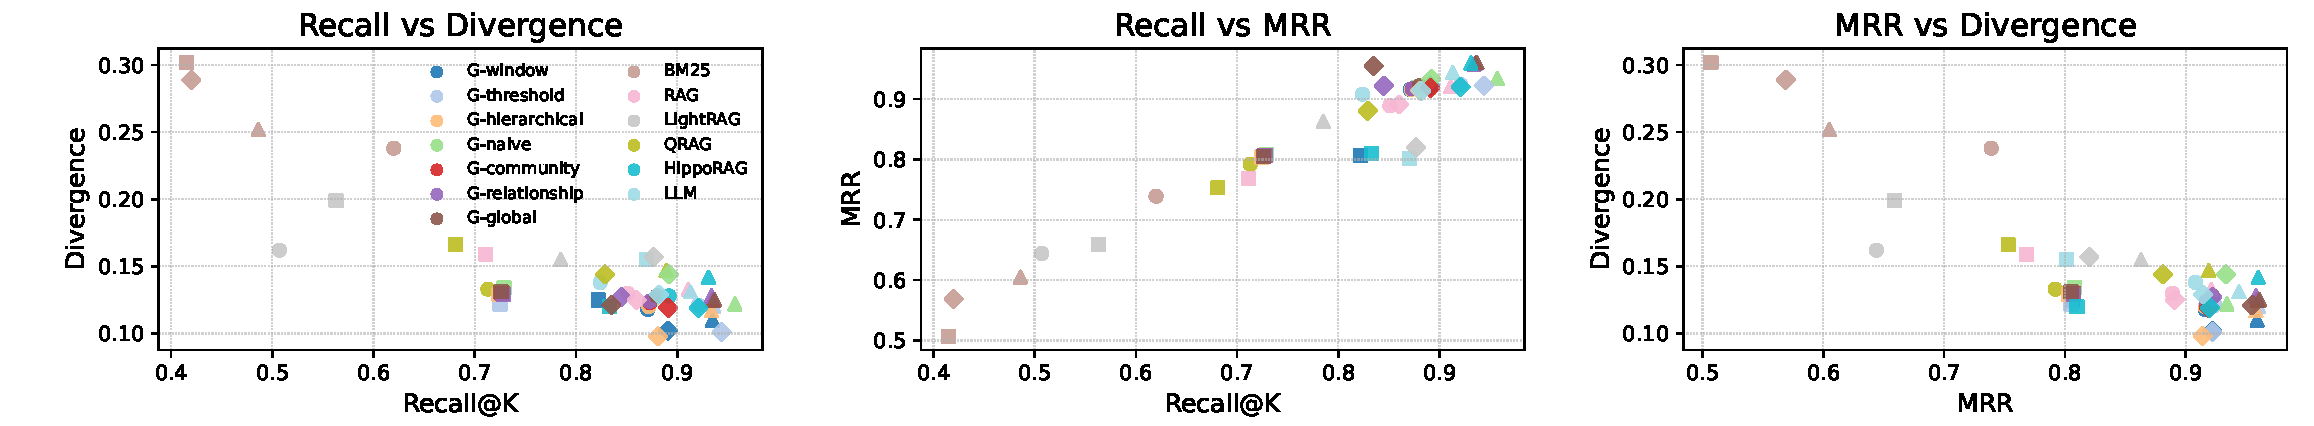
\includegraphics[width=0.95\linewidth]{figs/1_div_corr.pdf}
    \caption{Metric Correlations Across Datasets, Legend by Retriever}
    \label{fig:1_div_corr}
% \vspace{-1.5em}
\end{figure*}


% \vspace{-1em}
\subsection{Sensitivity of MI Hyperparameters (\textbf{RQ2})}
% \vspace{-0.5em}
\label{sec:hparam}
To address RQ2, we investigate the variation of the proposed MI based metric under different hyperparameter configurations. Specifically, we examine three key hyperparameters: 

(1) \textbf{MI candidate depth}: the top-$K$ to compute MI for each question, which is the length of $C_q$. We visualize a line sweep over the top-$K$, with value varies in $\{3, 5, 10, 20, 50, 100 \}$.

(2) \textbf{Anchor retriever}: the basis of supporting chunk list ($C_q$) that the divergence score is computed on top of. We consider two choices under this setting. (i) The union of all retrievers' chunk sets, which means that MI scores are computed on top of the union of all retriever chunks. (ii) One single retriever. In practice we implemented HippoRAG as the anchor of $C_q$, so that top-$K$ of HippoRAG's retrieved chunks are pulled as the basis for MI scores. Missing chunks from other retrievers are filled with zero values.


(3) \textbf{The reinforce strength coefficient} ($\gamma$ in Eq. \eqref{eq:CPasttilde}). It takes values from $\{2, 10, 100\}$.

We quantify the alignment of the recall and the negative divergence score using Pearson Correlation. The results on HotPotQA are plotted in Figure \ref{fig:2_hparam}, where the X-axis is the top-$K$ line sweep, and the legends are anchor retriever and $\gamma$.
% More results are shown in Appendix \ref{appendix:hparam}.



\begin{figure}[H]
    \centering
    \renewcommand{\thefigure}{2}
    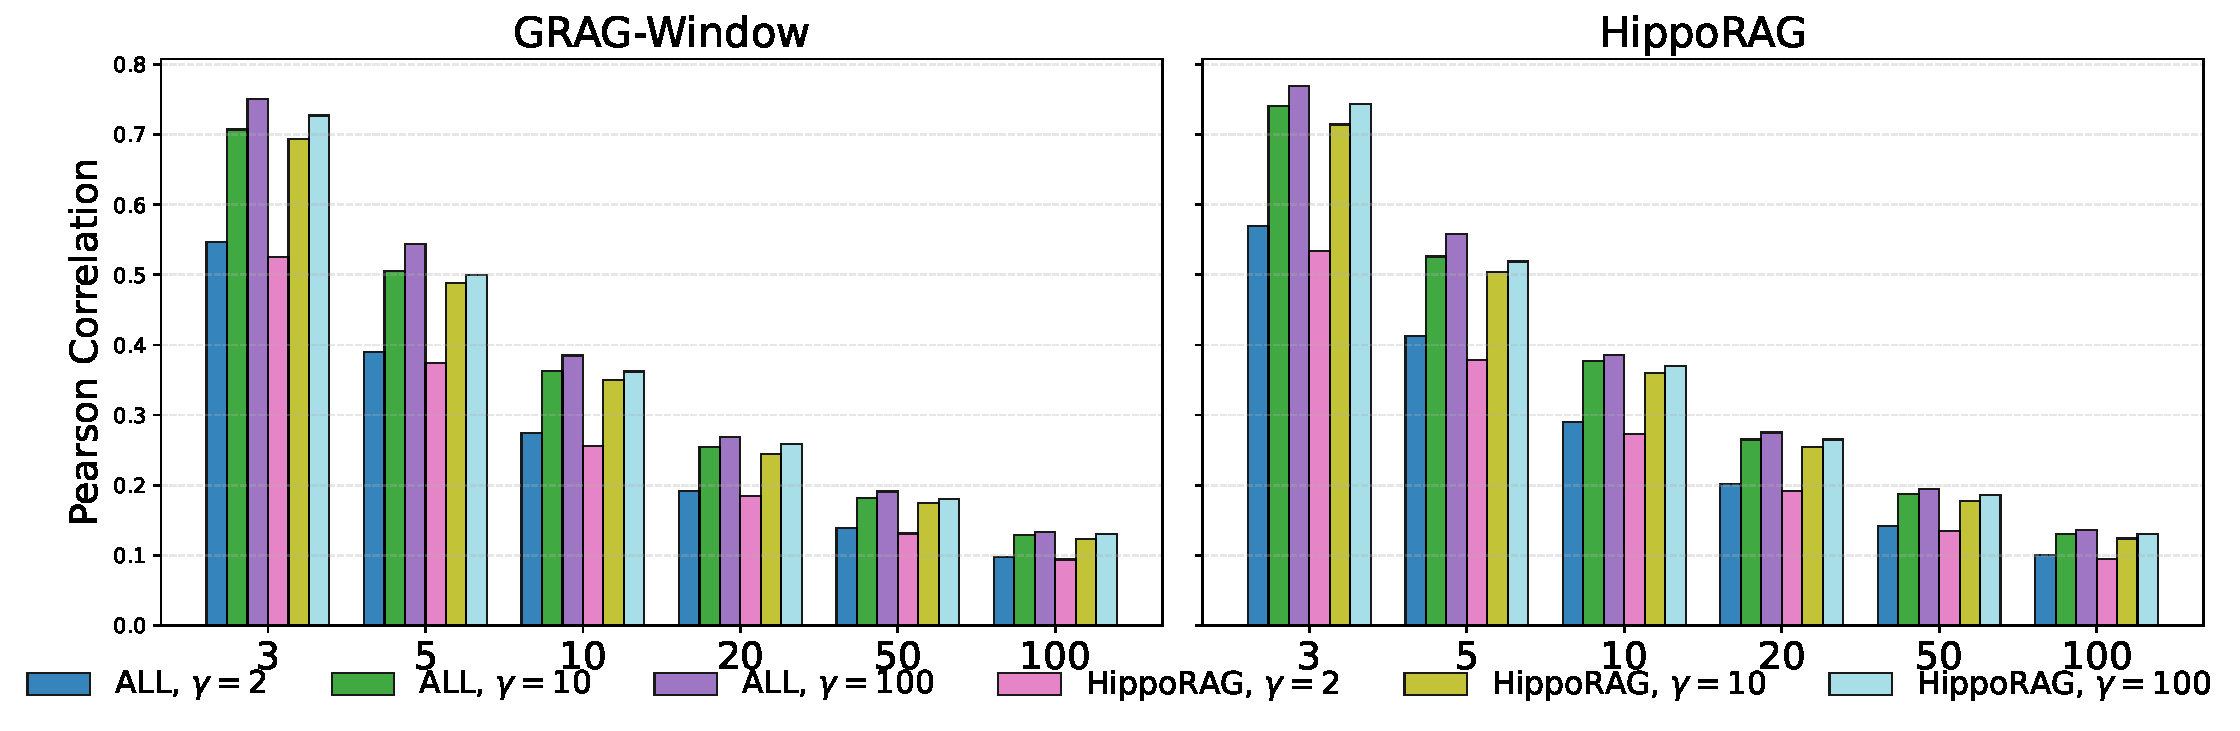
\includegraphics[width=0.97\linewidth]{figs/2_hparam.pdf}
    \caption{Hparam robustness visualization. Using the first bar of the first subfigure (RAG) to interpret the meaning: in HotPotQA dataset and for GRAG-Window retriever, the Pearson correlation between the \textit{Div} metric and the Recall is 0.54 if the \textit{Div} is computed at top 3 chunks retrieved by all retrievers (otherwise, top 3 chunks retrieved only by HippoRAG) and $\gamma$ is set to 2 for the \textit{Div}.}
    \label{fig:2_hparam}
    % \vspace{-1em}
\end{figure}

The first observation is that large $\gamma$ brings up the correlation values. This is because large $\gamma$ will degenerate the pseudo ground truth into one hot (or few-hot for multi-hop QA) labels. In that case, the divergence is mainly capturing the entropy on the golden chunks, bringing up its correlation with recall.


We also observe that as top-$K$ increases, the Pearson correlation generally decreases, as reflected by all lines showing a consistently decreasing trend. This suggests that the retrievers exhibit different distributions than the pseudo-ground truth distributions. Otherwise if the retriever distribution is similar to the pseudo-ground truth distribution except by picking the wrong peak (golden chunk), their distribution shift should gradually close as top-$K$ increases.




\subsection{Retriever Ensemble and Shapley Contribution Values (\textbf{RQ3})}

We conduct a series of experiments in the attempt to find a subset of combined retrievers outperforming any single strongest retriever, as well as visualizing the synergy and redundancy across different retrievers.

Our retriever ensemble is based on the divergence metric. For every given dataset, we first run retrieval procedure with every retriever to get a large top-K chunk list for 1000 QA pairs. Then we select a list of retriever subset to perform ensemble search in the unified search space, then the best retriever ensemble algorithm is found within that space, using the 20\% training QA pairs. Finally, the ensembled retriever is evaluated on the test 80\% QA pairs. The detailed options for the retreiver ensemble algorithm space are specified in Appendix \ref{appendix:ranker fusion}.

We break down this research question into several key points for a better comprehensive understanding.


% \vspace{-0.5em}
\begin{itemize}
    % \vspace{-0.5em}
    \item \textbf{RQ3.1} How much are these retrievers contributing to the ensembled results?
    
    % \vspace{-0.5em}
    \item \textbf{RQ3.2} How much information does the best ensemble strategy provide? What if it deviates from the best configuration?

% \item \textbf{RQ3.3} Are the retriever relative contribution ratios staying the same across datasets?

    % \vspace{-0.5em}
    \item \textbf{RQ3.3} Ensemble stability: if more retrievers are added to the best ensemble configuration, or some retrievers are dropped, how does it impact the performance?
\end{itemize}
% \vspace{-1em}

\subsubsection{Best Recall by Shapley Shares (RQ3.1)}
% \vspace{-0.5em}
We compute the Shapley attribution values for every retriever within the best retriever set in Figure~\ref{fig:3_1_shapley}. The height of the bar plot means the overall recall performance relative to 1.0. From this figure we can see that the strongest retriever also tends to contribute the most. However, the winner is not the ensemble of the top-performing GraphRAG retrievers, but it often includes worse retrievers such as BM25. This hints that different GraphRAG retrievers may contain redundant components that harm synergy.

\begin{figure}[H]
    \centering
    \renewcommand{\thefigure}{3.1}
    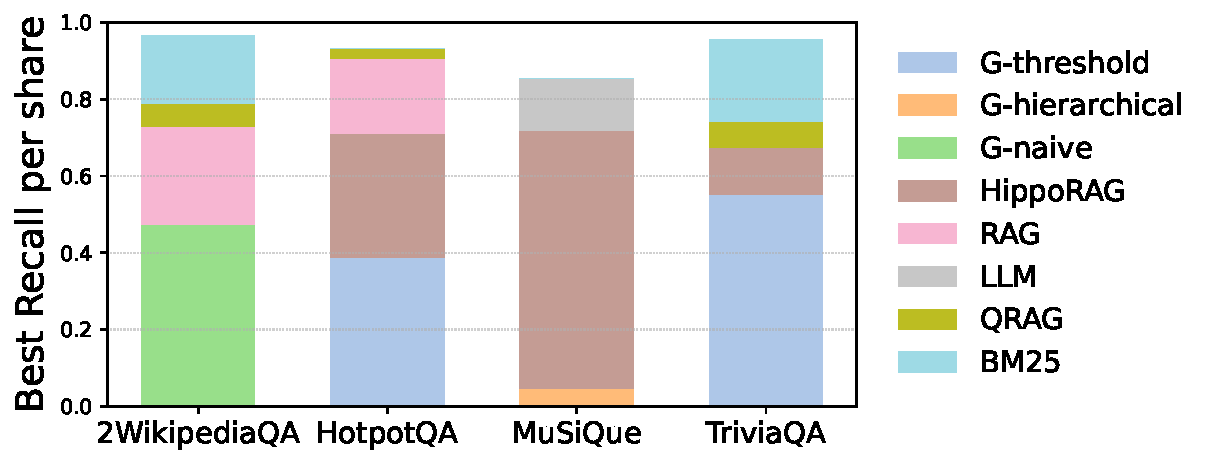
\includegraphics[width=1\linewidth]{figs/3_1_shapley.pdf}
    \caption{Shapley share for the best ensemble configs.}
    \label{fig:3_1_shapley}
    % \vspace{-0.5em}
\end{figure}


\subsubsection{Perturbation Impact on MI (RQ3.2)}

We evaluate RQ3.2 by computing $I(\widetilde{\mathrm{CP}}^\ast; X_S)$ from Eq.~\eqref{eq:util} for the best retriever subset and its perturbed variations, where $S$ is some retriever ensemble set. The results are plotted in Figure~\ref{fig:3_3_perturb}. In this figure, the y-axis labels are different retriever subsets, ranked by the MI. As can be seen in the figure, the few top performing retriever subsets show similar performance. However, when the perturbation of retrievers are too large, the performance drops drastically.

\begin{figure}[htbp]
    \centering
    \renewcommand{\thefigure}{3.3}
    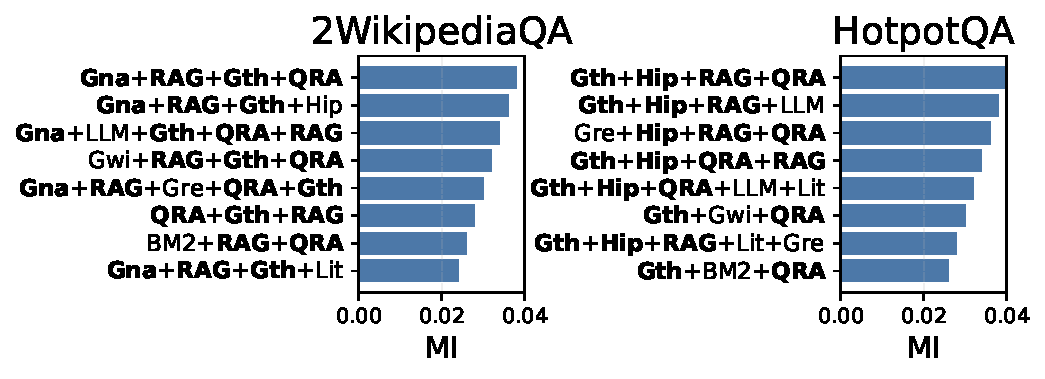
\includegraphics[width=0.97\linewidth]{figs/3_3_perturb.pdf}
    \caption{MI under ensemble perturbation.}
    % \vspace{-0.5em}
    \label{fig:3_3_perturb}
\end{figure}
% \vspace{-1em}

\subsubsection{Perturbation Impact on Recall (RQ3.3)}
% \vspace{-0.5em}

We answer RQ3.3 by first identifying the best retriever subset for ensemble, then gradually add or drop retrievers on top of this best subset, and finally concatenate all results into a continuous line. We plot the results in Figure~\ref{fig:3_2_drop_line}.
\begin{figure}[H]
    \centering
    \renewcommand{\thefigure}{3.2}
    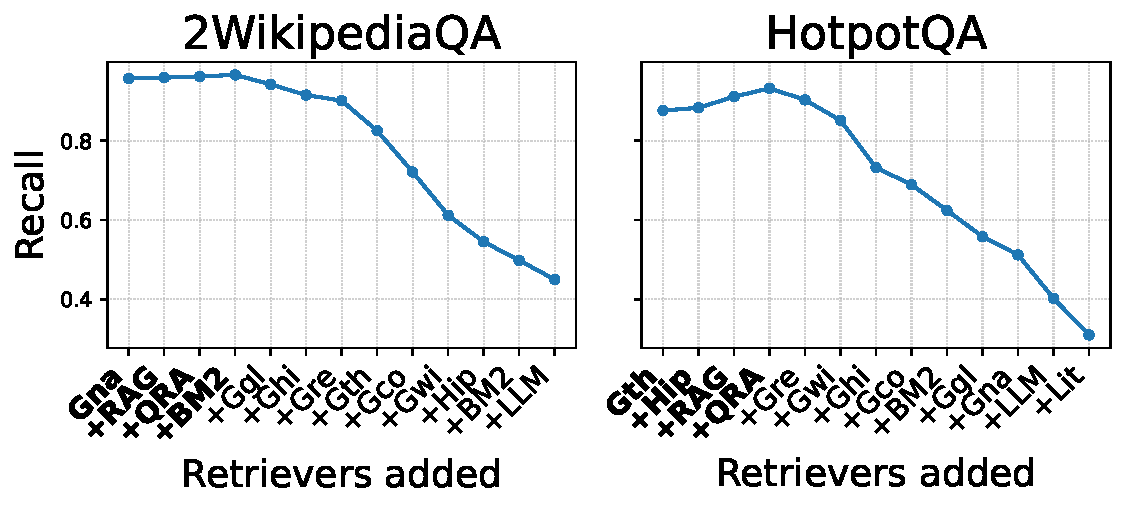
\includegraphics[width=0.9\linewidth]{figs/3_2_drop_line.pdf}
    \caption{Recall under ensemble perturbation.}
    % \vspace{-0.5em}
    \label{fig:3_2_drop_line}
\end{figure}


As can be seen in Figure~\ref{fig:3_2_drop_line}, if the retriever subset is chosen wisely, it performs better than single best retriever. As more retrievers are added, redundancy dominates over synergy, hence the performance dropped drastically.


% \subsubsection{Does retriever ensemble strategy generalize across datasets (RQ3.3)}

% \begin{figure}[H]
%     \centering
%     \renewcommand{\thefigure}{3.3}
%     \includegraphics[width=0.9\linewidth]{figs/3_3_crossds.pdf}
%     \caption{Cross-Dataset Generalization Results.}
%     \label{fig:3_3_crossds}
% \end{figure}

% By observing Figure~\ref{fig:3_3_crossds}, we see that the best configuration of retrievers are different across datasets, which means the best ensemble strategy are specific to the problem, and there is no single best retriever ensemble strategy that wins all cases. 





% \vspace{-1em}
\subsection{Retriever Redundancy Spectrum (RQ4)}
% \vspace{-0.5em}
\label{sec:spectrum}
We formulate the visualization of the $m$ retrievers as a geometric embedding problem. We first pre-compute the pairwise redundancy for all retrievers. By interpreting the pairwise redundancy as a measure of similarity, we derive a distance metric where highly redundant pairs correspond to short distances as in Eq. \ref{eq:dist def}. Using Classical Multidimensional Scaling (MDS), we map the high-dimensional relationship matrix into a 2D Euclidean space. This mapping preserves the global relational structure, allowing us to visualize retriever clusters based on their informational synergy, as shown in Figure \ref{fig:4_retriever_space}.

\begin{figure}[htbp]
    \centering
    \renewcommand{\thefigure}{4}
    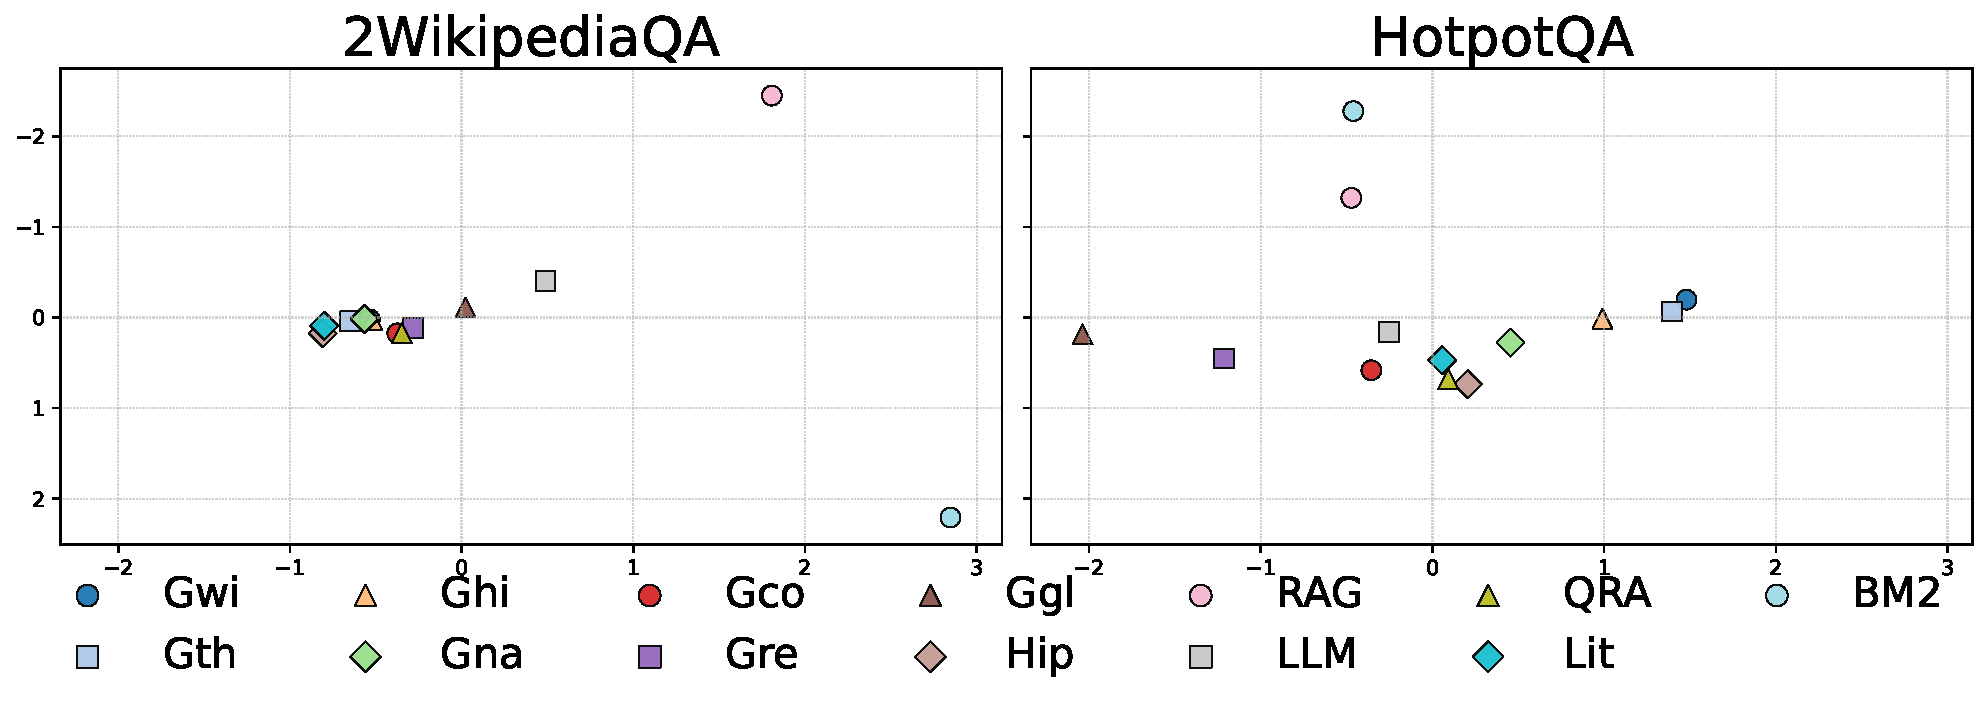
\includegraphics[width=0.97\linewidth]{figs/4_retriever_space.pdf}
    \caption{Retriever redundancy/synergy spectrum.}
    \label{fig:4_retriever_space}
\end{figure}

As can be observed in the figure, GraphRAG approaches are similar to each other and further away from vanilla RAG or lexical BM25 retriever. This implies that redundancy might be clustered by approach types (graph vs. lexical vs. vanilla).


% \vspace{-0.5em}
% \vspace{-0.5em}
\section{Conclusion And Limitations}

We introduced MIGRASCOPE, an information-theoretic framework for evaluating RAG retrievers using principled metrics that quantify quality, redundancy, synergy, and marginal contribution. By modeling rankings as noisy views of an answer-conditioned chunk distribution, our approach provides actionable insights for retriever selection and demonstrates that carefully designed ensembles can outperform individual retrievers. This work offers a fresh perspective on retrieval evaluation and contributes tools for building more robust and efficient RAG systems.

As a pioneering effort in applying mutual information to retriever evaluation, MIGRASCOPE has certain limitations that suggest opportunities for refinement. The MI-based metrics, while theoretically grounded, are less familiar than conventional metrics like Recall@K or MRR, and their interpretation may require additional context for practitioners. The framework depends on hyperparameters and estimator choices, which can influence numerical stability and relative rankings, though sensitivity analysis can mitigate these effects. Additionally, the reported MI values are approximations influenced by model assumptions, estimator errors, and practical truncations, and should be viewed as consistent estimates under specific settings.

Despite these limitations, MIGRASCOPE reveals new insights into retriever interactions and highlights the potential of ensemble methods. Future work could extend this framework to integrate generation-side metrics, explore retriever-specific internal mechanisms, and optimize computational efficiency for large-scale deployments. By addressing these directions, the community can build on this foundation to further advance retrieval-augmented generation systems.


% \section{Conclusion}

% We presented an information-theoretic framework that normalizes retriever evaluation through the lens of information theory. By modeling rankings as noisy views of an answer-conditioned chunk distribution, our MI-based metrics quantify quality, redundancy and marginal contribution, enabling principled selection and lightweight ensembles that outperform single retrievers and offer actionable guidance for robust and efficient RAG systems.
% % We hope these tools shift the focus from inventing new retrievers to understanding and composing existing ones.


% \section{Limitations}

% Despite its empirical utility, MIGRASCOPE has several limitations that qualify the scope of its conclusions and suggest directions for future work.

% \subsection{Units and Interpretability}
% The proposed mutual-information (MI) based metrics---including the divergence-derived retriever quality score and the redundancy/synergy measures---are expressed in bits or nats. While these units have clear information-theoretic meaning, they are less intuitive to practitioners compared to conventional retrieval metrics such as Recall@K, MRR, or NDCG. As a result, interpreting absolute magnitudes and setting actionable thresholds can be nontrivial. In practice, we recommend viewing MI-based scores as complementary diagnostics that expose dependence structure and marginal evidence, rather than as replacements for standard task metrics.

% \subsection{Sensitivity to Hyperparameters and Stability}
% Our MI estimates depend on multiple hyperparameters and estimator choices, which can influence numerical stability and relative rankings (see Section~\ref{sec:hparam}). 
% These knobs introduce bias--variance trade-offs; small changes may shift absolute MI values and, in edge cases, alter conclusions about redundancy or synergy. While cross-validation and sensitivity analysis mitigate these issues, the framework remains more fragile than purely rank-based metrics.

% \subsection{Approximation Rather Than Absolute Values}
% The MI quantities we report are typically approximations, not exact values, for several reasons:
% \begin{enumerate}
%     \item The presumed ideal relevance distribution derived from LLM guidance may not be an optimal estimator of the true chunk relevance probabilities. Any model misspecification or prompt bias propagates to MI estimates.
%     \item Because the score distribution over chunks is unknown and often high-dimensional, entropy and mutual information lack closed-form solutions. Estimators (density models, kNN, or neural estimators) introduce additional estimation error, including finite-sample bias and variance.
%     \item MI computation depends on hyperparameters such as the top-$K$ truncation. Theoretically, $K$ should cover all chunks; practically, large $K$ is computationally prohibitive, and long-tail distributions amplify variance. Truncation can therefore induce bias and sensitivity that must be balanced against runtime constraints.
% \end{enumerate}
% Consequently, the reported MI values should be interpreted as consistent estimates under stated settings, rather than absolute ground truth.

% \subsection{Scope Restricted to the Retrieval Layer}
% Our analysis treats retrievers as black-box mechanisms that provide chunk-level scores or probabilities and benchmarks only the retrieval step. We do not attempt to model or compare the internal inductive biases, architectures, or optimization strategies of individual retrievers. Extending the information-theoretic analysis to internal mechanisms would require retriever-specific abstractions and assumptions that substantially increase theoretical complexity and reduce generality.

% \subsection{Computational Cost and Scaling}
% Estimating MI at corpus scale is computationally demanding. Pairwise redundancy/synergy analyses scale with the number of retrievers, and multi-retriever interaction terms can grow combinatorially. Moreover, larger corpora, higher top-$K$, and more expressive estimators increase runtime and memory requirements. Although we employ practical truncations and batching, the framework may be costly for extremely large RAG deployments without additional approximation strategies.

% \subsection{Evaluation Scope Beyond Retrieval}
% Although the ensemble results indicate improved retrieval utility, our benchmarking focuses on the retriever component rather than full end-to-end generation quality. Downstream LLM behavior (faithfulness, formatting constraints, reasoning chains) can modulate the practical impact of retrieval improvements. Integrating MI-based diagnostics with generation-side metrics is left for future work.


% % \subsection{Dataset and Annotation Dependence}
% % Ground-truth answers and relevance judgments in existing RAG corpora can be noisy, incomplete, or biased toward particular knowledge styles (e.g., factual Q/A vs. multi-hop reasoning). MI-based attribution and synergy estimates are therefore contingent on dataset characteristics and annotation quality. Insights may not fully generalize to domains with different semantics, document structures, or retrieval goals.

% % \subsection{Visualization and Diagnostic Limits}
% % The proposed visual diagnostics summarize high-dimensional relationships between retrievers into low-dimensional plots. While useful for spotting overlap and complementarity, these visualizations may oversimplify interaction structure, obscure conditional dependencies, or overemphasize estimator artifacts. They should be used alongside quantitative sensitivity analyses.





\bibliography{example_paper}
\bibliographystyle{icml2026}

%%%%%%%%%%%%%%%%%%%%%%%%%%%%%%%%%%%%%%%%%%%%%%%%%%%%%%%%%%%%%%%%%%%%%%%%%%%%%%%
%%%%%%%%%%%%%%%%%%%%%%%%%%%%%%%%%%%%%%%%%%%%%%%%%%%%%%%%%%%%%%%%%%%%%%%%%%%%%%%
% APPENDIX
%%%%%%%%%%%%%%%%%%%%%%%%%%%%%%%%%%%%%%%%%%%%%%%%%%%%%%%%%%%%%%%%%%%%%%%%%%%%%%%
%%%%%%%%%%%%%%%%%%%%%%%%%%%%%%%%%%%%%%%%%%%%%%%%%%%%%%%%%%%%%%%%%%%%%%%%%%%%%%%
\newpage
\appendix
% \onecolumn









\section{Detailed RAG/GraphRAG Formulations}
\label{appendix:grag formulations}
This section formalizes the graph construction and retrieval variants used in our evaluation, emphasizing succinct definitions and avoiding redundant statements.

\subsection{Method 1: Windowed Co-occurrence Graph}
The \textbf{G-Window} method limits co-occurrence edges to entities within a fixed offset in the ordered entity list $\mathcal{E}_c$ for any chunk $c$.
\begin{small}
\begin{multline}
E_{\text{Window}} = \Bigl\{ \{e_i, e_j\} \mid e_i, e_j \in \mathcal{E}, \, i \neq j, \, 
\exists c \in C, \exists k, l : \\ 
(\mathcal{E}_{c,k} = e_i \land \mathcal{E}_{c,l} = e_j \land |k - l| \le \text{window\_size}) \Bigr\}
\end{multline}
\end{small}

\subsection{Method 2: Thresholded Co-occurrence Graph}
The \textbf{G-Threshold} method filters incidental co-occurrences by requiring a minimum count across the corpus:
\begin{multline}
    E_{\text{Threshold}} = \{\{e_i, e_j\} \mid e_i, e_j \in \mathcal{E}, i \neq j, \\ 
    \sum_{c \in C} \mathbf{I}(\{e_i, e_j\} \subseteq \mathcal{E}_c) \ge \text{min\_cooc} \}
\end{multline}

\subsection{Method 3: Hierarchical and Algorithmic Graph Construction Methods}
\textbf{G-Hierarchical} constructs a heterogeneous directed graph $G=(V, E)$ with document, chunk, and entity nodes, enabling explicit provenance.
\begin{itemize}
    \item $(\text{doc}:d, \text{chunk}:c)$ with $\text{type: CONTAINS}$.
    \item $(\text{chunk}:c, \text{entity}:e)$ with $\text{type: MENTIONS}$ for $e \in \mathcal{E}_c$.
    \item undirected $\{e_i, e_j\}$ with $\text{type: CO\_OCCURS}$ for $e_i, e_j \in \mathcal{E}_c$.
\end{itemize}

\subsection{Method 4: Naive Co-occurrence Graph}
\textbf{G-Naive} establishes an undirected edge between any two entities that co-occur in at least one chunk:
\begin{tiny}
\begin{equation}
E_{\text{Naive}} = \left\{ \{e_i, e_j\} \mid e_i, e_j \in \mathcal{E}, \, i \neq j, \, \exists c \in C : \{e_i, e_j\} \subseteq \mathcal{E}_c \right\}
\end{equation}
\end{tiny}

\subsection{Method 5: Community Graph}
\textbf{G-Community} first forms $G_{\text{temp}}=(\mathcal{E}, E_{\text{Threshold}})$, then applies Louvain to obtain clusters $\mathcal{S}_k$:
\begin{small}
\begin{equation}
\{\mathcal{S}_1, \mathcal{S}_2, \dots\} = \mathbf{Louvain}(G_{\text{temp}}, \text{weight: cooccurrence})
\end{equation}
\end{small}
Community nodes $v_k$ are added with edges $E_{\text{Comm}} = \{ (e, v_k) \mid e \in \mathcal{S}_k, \text{type: BELONGS\_TO} \}$.

\subsection{Method 6: Relationship Graph}
\textbf{G-Relationship-Global} focuses on relationships among significant entities $\mathcal{E}_{\text{sig}}$ (frequency $\ge \text{MIN\_ENTITY\_OCCURRENCE}$), aggregating their global context:
\begin{equation}
C_e = \{c \in C \mid e \in \mathcal{E}_c \}
\end{equation}
Directed relationships are extracted by an LLM over $\text{Context}(C_e)$:
\begin{small}
\begin{equation}
E_{\text{RelGlobal}} = \bigcup_{e \in \mathcal{E}_{\text{sig}}} \mathbf{LLM}_{\text{extract\_global}}(\text{Context}(C_e), e, \mathcal{E}_{\text{cand}})
\end{equation}
\end{small}

\subsection{Method 7: Global Co-occurrence Graph}
\textbf{G-Global} derives the corpus-level unique set of co-occurring entity pairs (i.e., the non-attributed, de-duplicated union of chunk-level co-occurrences; equivalent in edge set to Method 4 but without per-chunk metadata).

\subsection{Method 8: HippoRAG}
\textbf{HippoRAG} \cite{gutierrez2025rag} models an heterogeneous memory graph $G_{\text{mem}}=(V, E)$:
\begin{enumerate}
    \item \textbf{Graph Construction:} $V = \mathcal{E} \cup \mathcal{F} \cup C$, where $\mathcal{F}$ are OpenIE triples. Edges include containment and synonymy (via $\mathbf{Embed}$ similarity).
    \item \textbf{Fact Reranking:} Retrieve fact candidates $\mathcal{F}_{\text{cand}} = \mathbf{VDB}_{\mathcal{F}}(q)$ and refine with an LLM reranker:
    \begin{equation}
    \mathcal{F}_q = \mathbf{LLM}_{\text{Rerank}}(\mathcal{F}_{\text{cand}}, q)
    \end{equation}
    \item \textbf{PPR Initialization:} Extract query entities from $\mathcal{F}_q$ and form $\mathbf{p}_0$:
    \begin{equation}
    \mathbf{p}_0 = \mathbf{InitDistribution}(\mathbf{Map}_{\mathcal{F} \to \mathcal{E}}(\mathcal{F}_q))
    \end{equation}
    \item \textbf{PPR Graph Search:} Run PPR on $G_{\text{mem}}$:
    \begin{equation}
    \mathbf{PPR}_{\text{scores}} = \mathbf{PPR}(G_{\text{mem}}, \mathbf{p}_0)
    \end{equation}
    \item \textbf{Context Selection:} Select top-scoring chunks:
    \begin{equation}
    \mathcal{C}_q = \text{Top}_{k_C}(\{c_j\}_{j\in C}, \mathbf{PPR}_{\text{scores}}[c_j])
    \end{equation}
\end{enumerate}

\subsection{Method 9: RAG}
Standard RAG using embedding-based retrieval over chunks followed by generation.

\subsection{Method 10: LLM Reranking}
\textbf{LLM} reranking orders candidate chunks $\mathcal{C}_{\text{cand}}$ with the LLM:
\begin{equation}
R_{\mathbf{LLM}} = \mathbf{LLM}_{\text{rank}}(q, \mathcal{C}_{\text{cand}})
\end{equation}
The final context $\mathcal{C}_q$ is the top $k_C$ by $R_{\mathbf{LLM}}$. In our tests, candidates were produced via the windowed co-occurrence graph, but the reranker is graph-agnostic.

\subsection{Method 11: Question as Sub-chunk Summary (QRAG)}
\label{appendix:qrag}
\textbf{Graph Construction (Synthetic Questions).} For each chunk $c_i$, generate a set of synthetic questions:
\begin{equation}
\mathbf{Q}_i = \{q_{i, 1}, \dots, q_{i, M_i}\} = \mathbf{LLM}_{\text{Gen}}(c_i)
\end{equation}
\textbf{Retrieval Scoring.} Score $c_i$ by the maximum similarity between the query and its synthetic questions:
\begin{equation}
s_i = \max_{q_{i, j} \in \mathbf{Q}_i} \mathbf{Sim}(\mathbf{Embed}(q), \mathbf{Embed}(q_{i, j}))
\end{equation}
\textbf{Final Context.} Select the top $k$ chunks:
\begin{equation}
\mathcal{C}_q = \text{Top}_k(\{c_i\}_{i=1}^N, s_i)
\end{equation}

\subsection{Method 12: LightRAG}
\textbf{Graph Construction.} Build a directed, labeled graph $G_{\text{LightRAG}}=(\hat{\mathcal{E}}, \hat{\mathcal{R}})$ from LLM-extracted triples, applying deduplication and refinement:
\begin{equation}
G_{\text{LightRAG}} = \mathbf{Dedupe}\circ\mathbf{Prof}(\mathcal{V}_{\text{init}}, \mathcal{E}_{\text{init}})
\end{equation}
\textbf{Retrieval.} 
\begin{enumerate}
    \item \textbf{Search \& Neighborhood Expansion:} Retrieve $\mathcal{E}_{\text{sim}} = \mathbf{VDB}_{\mathcal{E}}(q)$, $\mathcal{R}_{\text{sim}} = \mathbf{VDB}_{\mathcal{R}}(q)$, then expand to $\mathcal{E}_{\text{hood}}$, $\mathcal{R}_{\text{hood}}$ via graph traversal.
    \item \textbf{Token Truncation:} Filter and truncate to a token budget $\mathbf{TB}$:
    \begin{small}
    \begin{multline}
    \mathcal{E}_{\text{final}}, \mathcal{R}_{\text{final}} = \\ \mathbf{Truncate}(\mathbf{Filter}(\mathcal{E}_{\text{sim}} \cup \mathcal{E}_{\text{hood}}, \mathcal{R}_{\text{sim}} \cup \mathcal{R}_{\text{hood}}), \mathbf{TB})
    \end{multline}
    \end{small}
    \item \textbf{Chunk Merging:} Map $\mathcal{E}_{\text{final}}, \mathcal{R}_{\text{final}}$ back to source chunks and merge.
    \item \textbf{Context Formatting:} Produce the final context:
    \begin{small}
    \begin{equation}
    \mathcal{C}_q = \mathbf{Format}(\mathcal{E}_{\text{final}}, \mathcal{R}_{\text{final}}, \mathbf{Merge}_{\mathcal{E}\mathcal{R} \to C}(\mathcal{E}_{\text{final}}, \mathcal{R}_{\text{final}}))
    \end{equation}
    \end{small}
\end{enumerate}

\subsection{Method 13: BM25}
Unmodified lexical BM25 retrieval.



\section{Ranker fusion}
\label{appendix:ranker fusion}

We formulate the ranker fusion search space as follows.

\paragraph{Score standardization.}
We apply per-retriever $z$-score normalization
\begin{multline}
\tilde{s}_i(c)=\frac{s_i(c)-\mu_i}{\sigma_i+\epsilon},\quad
\mu_i=\mathrm{mean}_c\,s_i(c),\\ \sigma_i=\mathrm{std}_c\,s_i(c).
\end{multline}

\paragraph{Weighted linear fusion.}
\begin{equation}
\hat{s}(c)=\sum_{i=1}^m w_i\,\tilde{s}_i(c),
\qquad
w_i\ge 0,\;\sum_i w_i=1.
\end{equation}
Weights can be set from divergence $w_i\propto \exp(-\lambda\,\mathrm{Div}(r_i))$, or learned by minimizing a surrogate loss such as cross-entropy to $\widetilde{\mathrm{CP}}^\ast$:
\begin{equation}
\min_{w}\; \sum_{q}\mathrm{CE}\!\Big(\widetilde{\mathrm{CP}}^\ast(\cdot\mid q,a_q),\;\mathrm{softmax}(\hat{s}(\cdot)/\tau)\Big).
\end{equation}

\paragraph{Temperature fusion of probabilities.}
Convert each retriever to a calibrated distribution
\begin{multline}
p_i(c\mid q)=\mathrm{softmax}\!\left(\frac{\tilde{s}_i(c)}{\tau_i}\right),
\\
\hat{p}(c\mid q)=\frac{\prod_{i=1}^m p_i(c\mid q)^{w_i}}{\sum_j \prod_{i=1}^m p_i(c_j\mid q)^{w_i}}
\end{multline}
which is a log-opinion pool.



\paragraph{Z-score fusion}
\begin{equation}
\phi_r(c)=\frac{s_r(c)-\mu_r}{\sigma_r+\epsilon},\qquad S(c)=\sum_{r=1}^m w_r\,\phi_r(c)
\label{eq:zscore}
\end{equation}
Z-score fusion \eqref{eq:zscore} aligns scales using per-list mean \(\mu_r\) and std \(\sigma_r\).

\paragraph{Logit pooling}
\begin{equation}
S(c)=\sum_{r=1}^m w_r\,\mathrm{logit}\!\big(\hat{p}_r(c)\big),\qquad \mathrm{logit}(p)=\log\frac{p}{1-p}
\label{eq:logit_fusion}
\end{equation}
Logit pooling \eqref{eq:logit_fusion} adds log-odds, equivalent to naive Bayesian evidence combination under independence.

\paragraph{Noisy-or}
\begin{equation}
\hat{p}(c)=1-\prod_{r=1}^m \big(1-\hat{p}_r(c)\big)^{w_r}
\label{eq:noisy_or}
\end{equation}
Noisy-or \eqref{eq:noisy_or} estimates the probability that at least one retriever deems \(c\) relevant.



\paragraph{Adaptive weights from divergence.}
\begin{equation}
w_r(q,a)=\frac{\big(\epsilon+\mathrm{Div}(r\mid q,a)\big)^{-1}}{\sum_{j=1}^m \big(\epsilon+\mathrm{Div}(j\mid q,a)\big)^{-1}}
\label{eq:weight_from_div}
\end{equation}
Inverse-divergence weights \eqref{eq:weight_from_div} emphasize better-aligned retrievers.





\paragraph{Reciprocal Rank Fusion (RRF).}
Let $\mathrm{rank}_i(c)$ be the rank of $c$ under $r_i$, then
\begin{equation}
\hat{s}(c)=\sum_{i=1}^m \frac{1}{k+\mathrm{rank}_i(c)},
\end{equation}
with $k>0$ controlling tail influence.

\paragraph{Borda count with weights.}
\begin{equation}
\hat{s}(c)=\sum_{i=1}^m w_i\big(|\mathcal{I}_q|-\mathrm{rank}_i(c)+1\big).
\end{equation}

\paragraph{Robust Rank Aggregation (RRA).}
For each $c$, compute a one-sided $p$-value under the null of random rankings,
\begin{multline}
p_i(c)=\frac{\mathrm{rank}_i(c)}{|\mathcal{I}_q|},\\
p_{\mathrm{agg}}(c)=\min_{t\in\{1,\dots,m\}} \mathrm{BetaCDF}\!\Big(p_{(t)}(c);\;t,\;m{-}t{+}1\Big),
\end{multline}
and rank by $- \log p_{\mathrm{agg}}(c)$.

\paragraph{Bayesian model averaging (BMA).}
Assuming per-retriever likelihoods $p_i(a\mid q,c)$ and model priors $\pi_i$, form
\begin{multline}
\hat{p}(c\mid q)\;\propto\;\sum_{i=1}^m \pi_i\, p_i(a\mid q,c)
\\ \text{or}\quad
\hat{s}(c)=\sum_i \log\big(\pi_i\, p_i(a\mid q,c)\big).
\end{multline}
If $p_i(a\mid q,c)$ is unavailable, use surrogates based on $\widetilde{\mathrm{CP}}^\ast$ or calibrated $p_i(c\mid q)$.

\paragraph{Markov-chain rank aggregation (Rank Centrality).}
Construct a transition matrix
\begin{equation}
M_{uv}=\frac{1}{Z}\sum_{i=1}^m \mathbf{1}[u\neq v]\cdot \sigma\!\big(\tilde{s}_i(v)-\tilde{s}_i(u)\big),
\end{equation}
with $\sigma(x)=1/(1+e^{-x})$ and row-normalization $Z$. The stationary distribution $\pi$ of $M$ defines the fused ranking by $\pi(c)$.






\section{Gaussian assumption.}
\label{appendix:gaussian assumption}

This section present an alternative way to estimate MI under vector observations in Section~\ref{sec:est MI under vec}. While the true distributions of the retriever scores $X$ and the pseudo ground truth scores $Y$ are unknown, adopting a Gaussian assumption facilitates computational tractability by making possible a closed-form solution.

Let \((Y,X_S)\) be jointly Gaussian with covariance
\(\Sigma=\begin{bmatrix}\Sigma_{YY} & \Sigma_{YX}\\ \Sigma_{XY} & \Sigma_{XX}\end{bmatrix}\).
\begin{equation}
H(Y)=\tfrac12\log\big((2\pi e)^{d_Y}\det\Sigma_{YY}\big).
\label{eq:H_gauss}
\end{equation}
\begin{equation}
\Sigma_{Y\mid X_S}=\Sigma_{YY}-\Sigma_{YX}\Sigma_{XX}^{-1}\Sigma_{XY}.
\label{eq:schur}
\end{equation}
\begin{equation}
H(Y\mid X_S)=\tfrac12\log\big((2\pi e)^{d_Y}\det\Sigma_{Y\mid X_S}\big).
\label{eq:H_cond_gauss}
\end{equation}
\begin{equation}
I(Y;X_S)=\tfrac12\log\frac{\det\Sigma_{YY}}{\det\Sigma_{Y\mid X_S}}.
\label{eq:I_gauss}
\end{equation}
Equations \eqref{eq:H_gauss}–\eqref{eq:I_gauss} use Schur complements to yield closed-form entropy and mutual information values.

Empirically, we observed that Gaussian assumption leads to MI values about one to two magnitude smaller, and the correlation with Recall is also lower, indicating over-simplification. We leverage the non-Gaussian assumption for MI estimation throughout this research.







\end{document}

% This document was modified from the file originally made available by
% Pat Langley and Andrea Danyluk for ICML-2K. This version was created
% by Iain Murray in 2018, and modified by Alexandre Bouchard in
% 2019 and 2021 and by Csaba Szepesvari, Gang Niu and Sivan Sabato in 2022.
% Modified again in 2023 and 2024 by Sivan Sabato and Jonathan Scarlett.
% Previous contributors include Dan Roy, Lise Getoor and Tobias
% Scheffer, which was slightly modified from the 2010 version by
% Thorsten Joachims & Johannes Fuernkranz, slightly modified from the
% 2009 version by Kiri Wagstaff and Sam Roweis's 2008 version, which is
% slightly modified from Prasad Tadepalli's 2007 version which is a
% lightly changed version of the previous year's version by Andrew
% Moore, which was in turn edited from those of Kristian Kersting and
% Codrina Lauth. Alex Smola contributed to the algorithmic style files.
